\documentclass[12pt,a4paper]{article}

% ===== Packages =====
\usepackage[utf8]{inputenc}        % Codificação UTF-8 para caracteres portugueses
\usepackage[T1]{fontenc}           % Codificação de fontes para português
\usepackage[portuguese,provide=*]{babel} % Hifenização e termos em português
\usepackage{geometry}              % Margens da página
\usepackage{graphicx}              % Inserção de imagens
\usepackage{hyperref}              % Links clicáveis no índice e referências
\usepackage{titlesec}              % Formatação dos títulos de secção
\usepackage{tocloft}               % Personalização do índice
\usepackage{fancyhdr}              % Cabeçalhos e rodapés personalizados
\usepackage{setspace}              % Espaçamento entre linhas
\usepackage{parskip}               % Espaço entre parágrafos em vez de indentação
\usepackage{enumitem}              % Personalização de listas
\usepackage{array}                 % Tabelas melhoradas
\usepackage{amsmath}               % Expressões matemáticas avançadas
\usepackage{tabularx}              % Tabelas com colunas ajustáveis à largura
\newcolumntype{Y}{>{\raggedright\arraybackslash}X}
\setlength{\tabcolsep}{8pt}        % Espaçamento horizontal das células da tabela
\renewcommand{\arraystretch}{1.5}  % Espaçamento vertical das linhas da tabela
\usepackage{booktabs}              % Linhas de tabela profissionais
\usepackage{makecell}              % Células com várias linhas em tabelas
\usepackage{float}                 % Força localização de floats com [H]
\usepackage{caption}               % Personalização de legendas
\usepackage{longtable}    
\usepackage{multirow}     
\usepackage{listings}              % Blocos de código fonte
\usepackage{listingsutf8}          % Suporte a ficheiros com codificação legacy em listings
\usepackage{xcolor}
\usepackage{float}
\usepackage[utf8]{inputenc}
\usepackage[T1]{fontenc}

% Definição de cores (baseadas na sua imagem)
\definecolor{codegray}{rgb}{0.95, 0.95, 0.92}
\definecolor{keywordcolor}{rgb}{0.8, 0.2, 0.2} % Vermelho para comandos
\definecolor{stringcolor}{rgb}{0.4, 0.4, 0.8}  % Azul para IDs/Nomes
\definecolor{commentcolor}{rgb}{0.5, 0.5, 0.5} % Cinza para comentários

\lstset{
    language=SQL,
    backgroundcolor=\color{codegray},
    basicstyle=\ttfamily\small,
    breaklines=true,
    keywordstyle=\color{keywordcolor}\bfseries,
    commentstyle=\color{commentcolor}\itshape,
    stringstyle=\color{stringcolor},
    showstringspaces=false,
    frame=none, % Se quiser borda, use 'single'
    tabsize=2,
    extendedchars=true,
    inputencoding=utf8,
    captionpos=b
}


% ===== Configuração de Margens =====
\geometry{
    top=2.5cm,
    bottom=2.5cm,
    left=3cm,
    right=2.5cm
}

% ===== Cor institucional UMinho =====
\definecolor{uminho}{RGB}{163, 31, 36}

% ===== Configuração de Hyperlinks =====
\hypersetup{
    colorlinks=true,
    linkcolor=black,
    urlcolor=uminho,
    citecolor=black,
    pdfauthor={Dinis Peixoto, Gonçalo Monteiro, Gonçalo Soares, José Novais, Rafaela Antunes},
    pdftitle={Título do Trabalho}
}

% ===== Espaçamento entre linhas =====
\onehalfspacing

% ===== Configuração dos cabeçalhos/rodapés =====
\pagestyle{fancy}
\fancyhf{}
\fancyfoot[C]{\thepage}
\renewcommand{\headrulewidth}{0pt}

% ===== Numeração das páginas iniciais em romano =====
% (será alternado ao longo do documento)

% =====================================================
% INÍCIO DO DOCUMENTO
% =====================================================
\begin{document}

% Evita âncoras duplicadas do hyperref enquanto a numeração é reiniciada
\hypersetup{pageanchor=false}

% =====================================================
% PÁGINA DE CAPA
% =====================================================
\begin{titlepage}
    \centering

    \vspace*{1cm}

    % Logo da Universidade do Minho
    
\includegraphics[width=0.25\textwidth]{images/logo_uminho.png}

    \vspace{0.3cm}
    {\large \textbf{Universidade do Minho}}\\[0.1cm]
    {\normalsize Licenciatura em Ciências da Computação}

    \vspace{3cm}

    {\large \textcolor{gray}{Unidade Curricular de Bases de Dados}}\\[0.3cm]
    {\large \textcolor{gray}{2025/2026}}

    \vspace{2.5cm}

    {\LARGE \textbf{Feira de Emprego Nacional da Universidade do Minho}}

    \vfill

    \vspace{0.8cm}

    \begin{minipage}{0.86\textwidth}
        \centering
        {\large\scshape Equipa de Trabalho}\\[0.35cm]
        {\Large\bfseries Dinis Peixoto a108566\\[0.12cm]
        Gonçalo Monteiro a108659\\[0.12cm]
        Gonçalo Soares a108393\\[0.12cm]
        José Novais a108395\\[0.12cm]
        Rafaela Antunes a102527}\\[0.6cm]
        {\normalsize\textit{Maio de 2026}}
    \end{minipage}

    \vspace{1cm}
\end{titlepage}

% =====================================================
% RESUMO (página numerada em romano)
% =====================================================
\pagenumbering{roman}
\setcounter{page}{1}

\section*{Resumo}
\addcontentsline{toc}{section}{Resumo}

\vspace{0.4cm}

\begin{minipage}{0.96\textwidth}
\small
Ao longo deste projeto foi desenvolvido um sistema de gestão de base de dados direcionado para a FENUM (Feira de Emprego Nacional da Universidade do Minho), com o objetivo de melhorar a organização e a gestão do evento. A solução permite centralizar informação sobre empresas participantes, estudantes, atividades e equipa organizadora, reduzindo redundâncias e facilitando a consulta dos dados.

O trabalho foi estruturado em várias fases, desde a definição do sistema e o levantamento de requisitos até à modelação conceptual, modelação lógica e implementação física. Para o desenvolvimento foram utilizadas as ferramentas BrModelo, na fase conceptual, e MySQL Workbench, na modelação lógica e na implementação física, garantindo uma transição coerente entre o modelo e a base de dados final.
\end{minipage}

\vspace{0.8cm}

\noindent\textbf{Palavras-chave:} Base de Dados, FENUM, Requisitos, Modelação Concetual, Modelação Lógica, Implementação Física.
\newpage

% =====================================================
% ÍNDICE GERAL
% =====================================================
\tableofcontents
\newpage

% =====================================================
% ÍNDICE DE FIGURAS
% =====================================================
\listoffigures
\newpage

% =====================================================
% ÍNDICE DE TABELAS
% =====================================================
\listoftables
\newpage

% =====================================================
% CORPO DO RELATÓRIO (numeração árabe)
% =====================================================
\hypersetup{pageanchor=true}
\pagenumbering{arabic}
\setcounter{page}{1}

% =====================================================
% 1. DEFINIÇÃO DO SISTEMA
% =====================================================
\section{Definição do Sistema}

\subsection{Contexto de aplicação}

A Feira de Emprego Nacional da Universidade do Minho (FENUM) teve a sua génese
em 2012, surgindo como uma resposta à necessidade de aproximar os estudantes de
Informática (antigamente FEIUM - Feira de Emprego de Informática da Universidade
do Minho) ao mercado de trabalho. O que começou como um pequeno evento de 15
empresas no átrio do Campus de Gualtar, expandiu-se, sob a coordenação do
Gabinete de Apoio ao Estudante, para um evento de escala nacional que hoje
abrange todas as áreas académicas da Universidade.

Nos últimos anos, a FENUM transformou-se num evento de grande dimensão, reunindo
centenas de empresas e milhares de estudantes. Esta evolução trouxe ganhos de
visibilidade para a Universidade e para os seus parceiros, mas também revelou
limitações operacionais críticas no modelo de gestão adotado até ao momento.

Atualmente, parte significativa da informação crítica continua dispersa por
formulários, folhas de cálculo e registos manuais. Esse cenário provoca atrasos
no atendimento, dificuldade em acompanhar candidaturas em tempo útil e um risco
acrescido de inconsistência de dados. Na prática, torna-se complexo responder
com rigor a perguntas fundamentais, como: que ofertas estão disponíveis, quem se
candidatou, que entrevistas ocorreram e quais os resultados obtidos.

Perante este contexto de crescimento, a criação de uma base de dados relacional
para a FENUM surge como uma necessidade estratégica. O sistema deverá
centralizar, organizar e validar os dados do evento, garantindo uma melhor
capacidade de coordenação entre estudantes, empresas e a equipa organizadora.

\subsection{Motivação e Objetivos do Trabalho}
\noindent A génese deste sistema reside na transição paradigmática de uma gestão de dados orgânica e reativa para uma solução de engenharia estratégica. Mais do que um repositório informativo, a arquitetura implementada visa a \textbf{erradicação da redundância} e a \textbf{preservação da integridade referencial}, garantindo que a escalabilidade do sistema acompanhe a crescente densidade logística da FENUM através de uma estrutura relacional rigorosa.

A motivação central desta infraestrutura foca-se na mitigação ativa dos riscos operacionais e anomalias de dados inerentes ao processamento manual e fragmentado. Ao consolidar fluxos de informação num esquema normalizado, assegura-se uma \textit{Single Source of Truth}, dotando a FENUM de uma infraestrutura robusta e resiliente, capaz de suportar o crescimento exponencial do evento e automatizar a tomada de decisão em edições futuras.

Os objetivos principais do sistema são:

\begin{itemize}[leftmargin=1.5cm]
    \item consolidar toda a informação sobre estudantes, empresas e dinâmicas da
    feira numa única fonte de verdade, assegurando a integridade referencial e
    eliminando a redundância de dados;
    \item reduzir falhas de registo e duplicação de informação, assegurando maior integridade dos dados;
    \item fornecer indicadores analíticos de desempenho (ex.: taxas de conversão
    de candidaturas, procura por setores de atividade), permitindo à organização
    da FENUM decisões baseadas em dados concretos;
    \item automatizar o agendamento de entrevistas e a gestão de lotação de
    palestras, minimizando conflitos de agenda e maximizando o aproveitamento do
    espaço;
    \item implementar políticas de controlo de acesso granulares, garantindo que
    cada interveniente (estudante, empresa, \textit{staff}) aceda apenas à
    informação necessária para a sua função;
    \item desenvolver um modelo de dados normalizado e resiliente, que sirva de
    alicerce para a gestão de edições futuras, garantindo a perenidade do
    sistema.
\end{itemize}

\subsection{Análise da Viabilidade do processo}

A viabilidade deste projeto sustenta-se num \textbf{tripé fundamental}: robustez
técnica, alinhamento organizacional e eficácia operacional.

Do ponto de vista técnico, o problema revela-se ideal para uma abordagem
relacional. A natureza do domínio, caracterizada por entidades bem definidas tais como \textit{Estudante}, \textit{Empresa}, \textit{Proposta} e \textit{Sessão} e relações claramente estruturadas, facilitou a modelação conceptual e a subsequente normalização até à \textbf{Terceira Forma Normal (3FN)}. 

Esta decisão de design é fundamental, pois a 3FN garante que cada atributo não-chave dependa exclusivamente da chave primária de forma direta e não transitiva. Na prática, esta rigorosa normalização permite eliminar redundâncias informativas e mitigar anomalias de inserção, atualização e remoção, assegurando que cada facto é armazenado num único local lógico da base de dados. Desta forma, a arquitetura FENUM transita de um modelo de gestão reativo para uma infraestrutura de dados estratégica, escalável e resiliente a inconsistências. As regras de negócio identificadas são objetivas e unívocas,
o que permite uma implementação lógica sem ambiguidades, assegurando a
integridade e a consistência dos dados desde a fase de desenho.

Do ponto de vista organizacional, o risco de desvio face aos objetivos reais da
FENUM é mitigado pela proximidade com os intervenientes do evento. A equipa
detém acesso direto às fontes de informação primária (documentação de suporte,
atas de reunião e recolha de requisitos), garantindo que o sistema desenvolvido
corresponda exatamente às necessidades de coordenação da organização.

Quanto à viabilidade operacional, o projeto apresenta um rácio custo-benefício
altamente favorável. A transição de registos fragmentados para uma solução
centralizada irá traduzir-se numa redução drástica dos tempos de atendimento,
numa melhor rastreabilidade das candidaturas e numa capacidade acrescida de
monitorização e auditoria em tempo real. Conclui-se, portanto, que a
implementação é tecnicamente exequível, organizacionalmente sustentada e
funcionalmente justificada pela criação de valor imediato para o evento.

\subsection{Recursos e Equipa de Trabalho}

Para a execução do projeto, foram considerados os seguintes recursos:

\begin{itemize}[leftmargin=1.5cm]
    \item \textbf{Recursos humanos:} equipa do projeto, elementos da organização
    da FENUM, estudantes participantes e representantes de empresas parceiras;
    \item \textbf{Recursos tecnológicos:} ferramentas de modelação (brModelo e
    MySQL Workbench), sistema de gestão de base de dados relacional e
    repositório de documentação do projeto;
    \item \textbf{Recursos documentais:} enunciado do trabalho, resultados de
    inquéritos, atas de reuniões e requisitos funcionais validados.
\end{itemize}

No âmbito da FENUM, foi formalmente criado o \textbf{Departamento de Gestão de
Base de Dados da FENUM}, responsável pela governação e manutenção da informação
do evento. Este departamento é composto por:

\begin{itemize}[leftmargin=1.5cm]
    \item \textbf{Diana Sameiro} (Diretora de Projeto e Analista de Requisitos):
    responsável pela interface entre o departamento e a FENUM, garantindo que os
    requisitos de negócio são traduzidos com rigor para o modelo de dados.
    \item \textbf{Bruno Jardim} (Arquiteto de Dados): responsável pela conceção
    do modelo conceptual e lógico, normalização da estrutura e garantia da
    integridade referencial do sistema.
    \item \textbf{Paulo Cartas} (Administrador de Base de Dados - DBA):
    responsável pela implementação física, configuração de políticas de
    segurança, gestão de acessos e monitorização de performance do SGBD.
\end{itemize}

Este departamento passa a assumir a responsabilidade pela coordenação das
operações de dados da feira, incluindo validação de requisitos, qualidade da
informação e articulação com as equipas funcionais.

\subsection{Plano de Execução do Projeto}

A execução do projeto seguiu uma metodologia faseada, organizada de forma a
garantir a evolução progressiva da solução desde a definição inicial do sistema
até à consolidação final da documentação. O trabalho decorreu entre
\textbf{17/04/2026} e \textbf{14/05/2026}, tendo sido acompanhado através do
Diagrama de Gantt apresentado na Figura~\ref{fig:gantt}.

\begin{figure}[H]
    \centering
    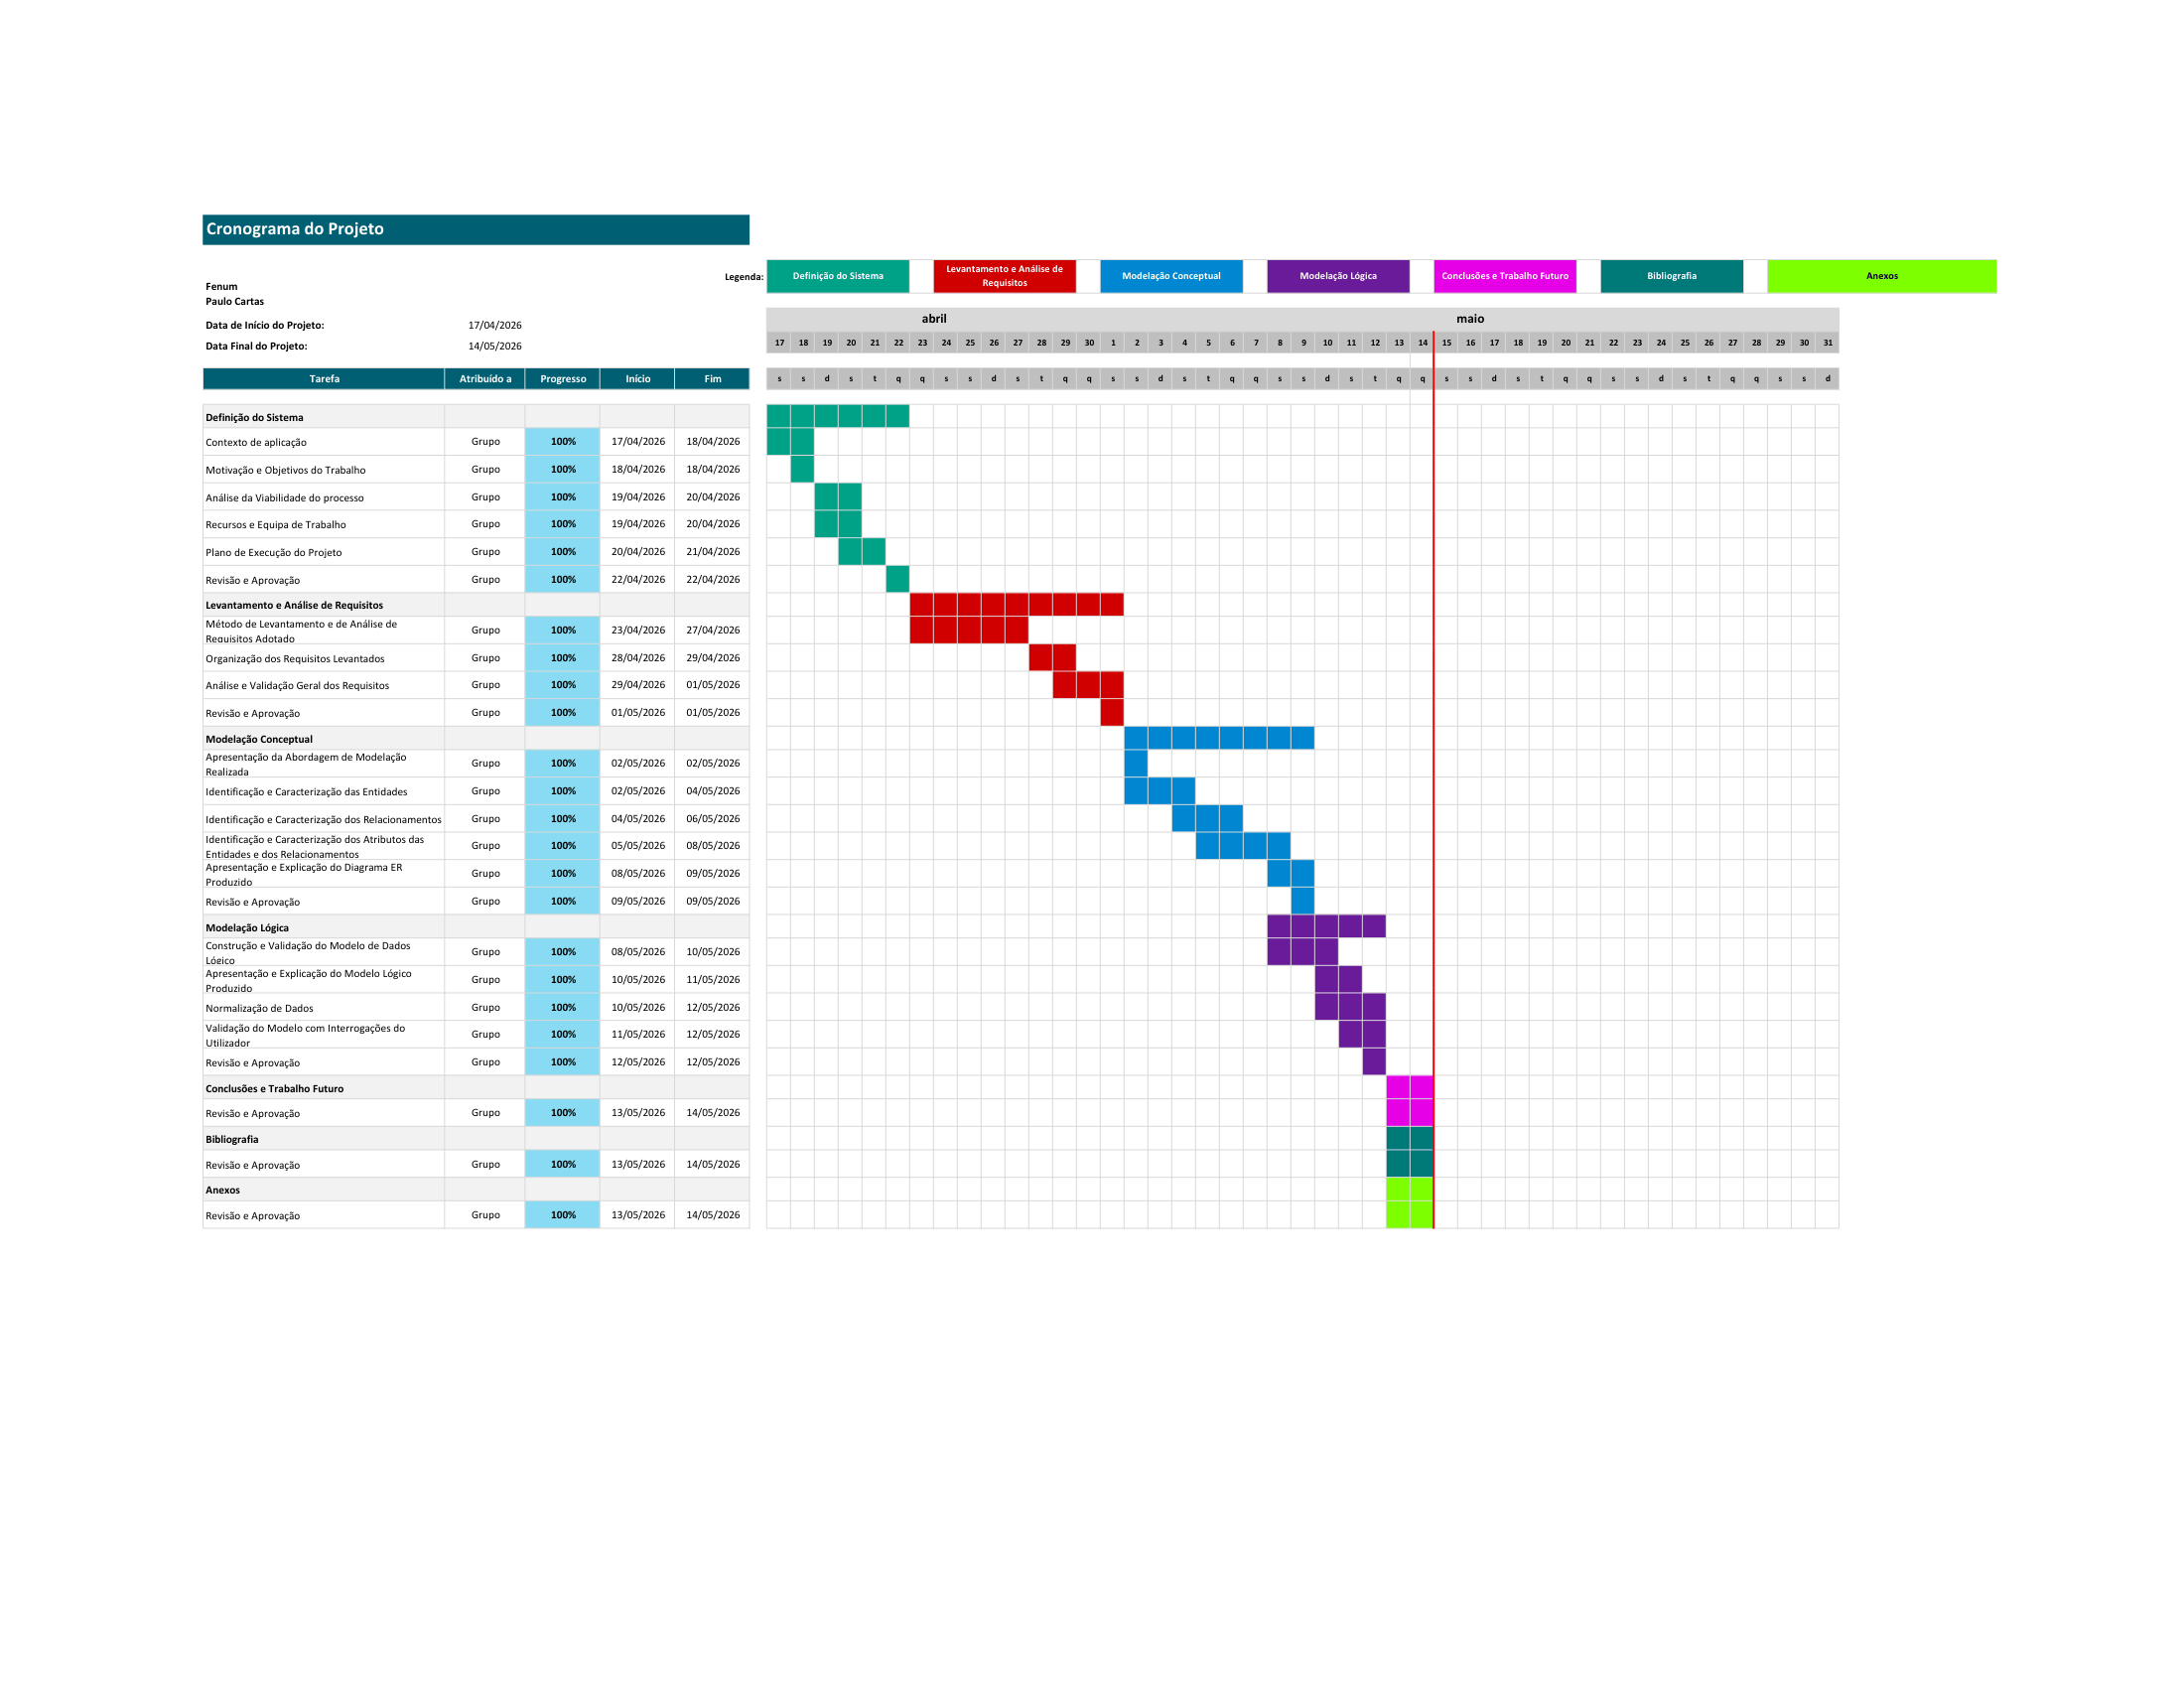
\includegraphics[width=\textwidth]{images/diagramaDeGantt-1.png}
    \caption{Diagrama de Gantt do projeto}
    \label{fig:gantt}
\end{figure}

O cronograma foi dividido em fases sequenciais, com alguns momentos de
sobreposição controlada quando as tarefas eram complementares. Esta organização
permitiu distribuir o esforço da equipa, acompanhar o progresso de cada etapa e
garantir que as decisões tomadas numa fase eram validadas antes de avançar para
a seguinte.

As fases principais do plano de execução foram as seguintes:

\begin{itemize}[leftmargin=1.5cm]
    \item \textbf{Definição do Sistema:} enquadramento do problema,
    identificação dos objetivos, análise de viabilidade, definição dos recursos
    necessários e validação inicial do plano de trabalho.
    \item \textbf{Levantamento e Análise de Requisitos:} escolha do método de
    levantamento, organização dos requisitos recolhidos, análise geral e revisão
    da sua adequação aos objetivos da FENUM.
    \item \textbf{Modelação Conceptual:} definição da abordagem de modelação,
    identificação das entidades, relacionamentos e atributos, culminando na
    produção e validação do Diagrama Entidade-Relacionamento.
    \item \textbf{Modelação Lógica:} conversão do modelo conceptual para o
    modelo lógico, normalização dos dados e validação do modelo com interrogações
    representativas do utilizador.
    \item \textbf{Conclusões, Bibliografia e Anexos:} consolidação final do
    relatório, revisão da documentação produzida e organização dos elementos
    complementares do projeto.
\end{itemize}

Em cada transição de fase, foram previstos momentos de revisão de qualidade para
assegurar a coerência entre o problema identificado e a solução modelada,
minimizando o risco de desalinhamento operacional. O acompanhamento contínuo do
cronograma permitiu gerir o esforço da equipa e garantir que os contributos de
todas as partes envolvidas foram integrados atempadamente no desenvolvimento da
solução.

% =====================================================
% 2. LEVANTAMENTO E ANÁLISE DE REQUISITOS
% =====================================================
\section{Levantamento e Análise de Requisitos}

\subsection{Método de Levantamento e de Análise de Requisitos Adotado}

O levantamento de requisitos seguiu um paradigma de \textbf{Desenvolvimento
Orientado a Artefactos}, garantindo que cada necessidade do negócio fosse
formalmente documentada, rastreável e validada. Esta abordagem visa eliminar a
subjetividade e assegurar a completa integridade entre as expectativas da FENUM
e o modelo lógico de dados final.

A metodologia estruturou-se em quatro pilares fundamentais:

\begin{itemize}[leftmargin=1.5cm]
    \item \textbf{Reuniões de descoberta e alinhamento:} sessões de alinhamento
    com a organização da FENUM e representantes de empresas. O foco não foi
    apenas a recolha de informação, mas a compreensão dos processos as-is e a
    definição dos processos to-be . Todas as decisões foram consignadas em atas
    de reunião.
    \item \textbf{Análise documental:} Estudo rigoroso dos formulários, folhas
    de cálculo e registos manuais utilizados anteriormente. Este método permitiu
    identificar campos críticos, redundâncias e a estrutura de dados existente
    que necessitava de normalização.
    \item \textbf{Levantamento por cenários de uso:} Tradução das necessidades
    em User Stories, técnica que permitiu a validação funcional rápida com o
    cliente e facilitou a comunicação entre o Departamento de Gestão de BD e a
    equipa funcional.
    \item \textbf{Validação Incremental e Controlo da Mudança:} Revisões
    periódicas onde os requisitos foram validados contra o enunciado do projeto.
    Qualquer alteração aos requisitos foi gerida de forma conservadora,rigorosa e controlada, garantindo
    que a base de dados evolui de forma consistente, evitando o 'scope creep'.
\end{itemize}

Para assegurar a eficiência operacional, a participação nas reuniões foi
otimizada conforme a necessidade dos tópicos em discussão, garantindo que o
conhecimento técnico e de negócio convergiu sempre para a mesma visão
estratégica.
\subsection{Organização dos Requisitos Levantados}

Com base no levantamento efetuado, os requisitos foram organizados em três
grupos: \textbf{descrição}, \textbf{manipulação} e \textbf{controlo}. Para
facilitar a implementação posterior, cada requisito foi reescrito no formato de
\textit{user story}.

\subsubsection{Matriz de rastreabilidade (requisito, fonte e reunião)}

A Tabela~\ref{tab:rastreabilidade} apresenta a ligação entre os requisitos
levantados e a respetiva origem nas reuniões (atas), permitindo justificar cada
item de forma auditável.

\begin{table}[H]
    \centering
    \caption{Rastreabilidade dos requisitos por reunião e fonte}
    \label{tab:rastreabilidade}
    \tiny
    \begin{tabular}{|l|l|p{5.5cm}|l|l|}
        \hline
        \textbf{ID} & \textbf{Tipo} & \textbf{Descrição resumida} & \textbf{Fonte} & \textbf{Data} \\
        \hline
        \multicolumn{5}{|c|}{\textbf{Requisitos de Descrição}} \\
        \hline
        RD01 & Descrição & Gestão de Estudantes (registo com identificador único). & Ata I & 01/03/2026 \\
        \hline
        RD02 & Descrição & Gestão de Empresas (registo com setor de atividade). & Ata II & 04/03/2026 \\
        \hline
        RD03 & Descrição & Gestão de Propostas (estágio/emprego/projeto). & Ata II & 04/03/2026 \\
        \hline
        RD04 & Descrição & Gestão de Palestras (sessões com dados logísticos). & Ata II & 04/03/2026 \\
        \hline
        RD05 & Descrição & Inscrições em Palestras (controlo de participação). & Ata II & 04/03/2026 \\
        \hline
        RD06 & Descrição & Candidaturas e Ofertas (rastreamento de candidatos). & Ata II & 04/03/2026 \\
        \hline
        RD07 & Descrição & Speed Interviews (registar e acompanhar contacto). & Ata III & 08/03/2026 \\
        \hline
        RD08 & Descrição & Gestão de STAFF (membros da equipa organizadora). & Ata III & 08/03/2026 \\
        \hline
        RD09 & Descrição & Gestão de Bancas (alocação de espaço físico). & Ata III & 08/03/2026 \\
        \hline
        RD10 & Descrição & Gestão de Oradores (identificador exclusivo e associação a empresa). & Ata III & 08/03/2026 \\
        \hline
        \multicolumn{5}{|c|}{\textbf{Requisitos de Manipulação}} \\
        \hline
        RM01 & Manipulação & Gestão de Candidaturas (atualizar estado das candidaturas recebidas). & Ata III & 08/03/2026 \\
        \hline
        RM02 & Manipulação & Estudantes Sem Candidaturas (listar estudantes sem atividade de recrutamento). & Ata III & 08/03/2026 \\
        \hline
        RM03 & Manipulação & Oradores com Múltiplas Palestras (listar oradores com mais do que uma palestra). & Ata III & 08/03/2026 \\
        \hline
        RM04 & Manipulação & Gestão de Estudantes (inserir, alterar ou apagar registos). & Ata III & 08/03/2026 \\
        \hline
        RM05 & Manipulação & Resultado de \textit{Speed Interview} (atualizar resultado após realização). & Ata III & 08/03/2026 \\
        \hline
        RM06 & Manipulação & Atribuição de Banca a Empresa (atribuir e consultar banca no recinto). & Ata III & 08/03/2026 \\
        \hline
        RM07 & Manipulação & Agenda Diária do Estudante (consultar palestras e \textit{speed interviews}). & Ata IV & 14/03/2026 \\
        \hline
        RM08 & Manipulação & Consulta de \textit{Speed Interviews} por Empresa (listar entrevistas agendadas). & Ata IV & 14/03/2026 \\
        \hline
        RM09 & Manipulação & Consulta de Procura de Propostas (dez propostas com mais candidaturas). & Ata IV & 14/03/2026 \\
        \hline
        RM10 & Manipulação & Empresas sem Candidaturas Recebidas (identificar propostas sem candidaturas). & Ata IV & 14/03/2026 \\
        \hline
        \multicolumn{5}{|c|}{\textbf{Requisitos de Controlo}} \\
        \hline
        RC01 & Controlo & Controlo da Organização (criar e alterar palestras, salas e oradores). & Ata IV & 14/03/2026 \\
        \hline
        RC02 & Controlo & Permissões de Empresas (ver apenas as suas próprias candidaturas). & Ata IV & 14/03/2026 \\
        \hline
        RC03 & Controlo & Permissões de Estudantes (ver ofertas e submeter candidaturas/inscrições próprias). & Ata IV & 14/03/2026 \\
        \hline
        RC04 & Controlo & Atribuição dos Espaços (atribuir bancas e gerir o espaço do evento). & Ata IV & 14/03/2026 \\
        \hline
    \end{tabular}
\end{table}

\subsubsection{Requisitos de Descrição (User Stories)}

\begin{itemize}[leftmargin=1.5cm]
    \item \textbf{US-RD01: Gestão de Estudantes} Como organização, quero registar cada
    estudante com identificador único, dados académicos e contacto, para
    garantir identificação inequíavoca.
    \begin{itemize}[leftmargin=1.2cm]
        \item \textbf{Atributos:} Num. Mecanográfico, Nome, E-mail, Curso, Universidade, Ano Letivo, Competências, Áreas de Interesse.
    \end{itemize}
    \item \textbf{US-RD02: Gestão de Empresas} Como organização, quero registar cada
    empresa com identificador único e setor de atividade, para permitir uma
    gestão estruturada das entidades empregadoras.
    \begin{itemize}[leftmargin=1.2cm]
        \item \textbf{Atributos:} ID Empresa, Nome, Setor, E-mail, Telefone, Banca Alocada.
    \end{itemize}
    \item \textbf{US-RD03: Gestão de Propostas} Como representante de empresa, quero registar
    propostas de estágio, emprego ou projeto com descrição e perfil pretendido,
    para divulgar oportunidades aos estudantes.
    \begin{itemize}[leftmargin=1.2cm]
        \item \textbf{Atributos:} ID Proposta, Título, Descrição, Tipo (Estágio/Emprego/Projeto), Perfil Procurado.
    \end{itemize}
    \item \textbf{US-RD04: Gestão de Palestras} Como organização, quero registar sessões de palestras com dados logísticos, para controlar a oferta formativa.
    \begin{itemize}[leftmargin=1.2cm]
        \item \textbf{Atributos:} ID Palestra, Sala, Lotação Máxima, Título, Orador, Data, Hora Início, Hora Fim.
    \end{itemize}
    \item \textbf{US-RD05: Inscrições em Palestras} Como estudante, quero inscrever-me em palestras, para garantir o meu lugar nas sessões de interesse.
    \begin{itemize}[leftmargin=1.2cm]
        \item \textbf{Atributos:} ID Inscrição, ID Aluno, ID Palestra, Estado (Confirmado/Lista de Espera).
    \end{itemize}
    \item \textbf{US-RD06: Candidaturas e Ofertas} Como estudante, quero candidatar-me a uma proposta, para participar nos processos de avaliação.
    \begin{itemize}[leftmargin=1.2cm]
        \item \textbf{Atributos:} ID Candidatura, ID Aluno, ID Oferta, Estado (Submetido/Análise/Aceite).
    \end{itemize}
    \item \textbf{US-RD07: Speed Interviews} Como organização, quero registar sessões
    de \textit{speed interview} com data e hora, para acompanhar o contacto
    direto entre estudantes e empresas.
    \begin{itemize}[leftmargin=1.2cm]
        \item \textbf{Atributos:} ID Entrevista, ID Aluno, ID Empresa, Data, Hora, Resultado.
    \end{itemize}
    \item \textbf{US-RD08: Gestão de STAFF} Como organização, quero registar os membros da equipa, para assegurar a coordenação operacional.
    \begin{itemize}[leftmargin=1.2cm]
        \item \textbf{Atributos:} ID Staff, Nome, Contacto, E-mail, Função.
    \end{itemize}
    \item \textbf{US-RD09: Gestão de Bancas} Como organização, quero associar cada
    empresa a uma ou mais bancas no recinto, para controlar a alocação física do espaço
    da feira.
    \begin{itemize}[leftmargin=1.2cm]
        \item \textbf{Atributos:} ID Banca, Código Banca, Zona, ID Empresa.
    \end{itemize}
    \item \textbf{US-RD10: Gestão de Oradores} Como organização,
    quero cadastrar oradores com um identificador exclusivo e associá-los obrigatoriamente a uma organização,
para que a agenda do evento reflita corretamente a representação corporativa e os oradores sejam validados de forma única no acesso às sessões.
    \begin{itemize}[leftmargin=1.2cm]
        \item \textbf{Atributos:} ID Orador, Nome, email, ID Empresa, \textit{linkedIn} e profissão.
    \end{itemize}
\end{itemize}

\subsubsection{Requisitos de Manipulação (User Stories)}

\begin{itemize}[leftmargin=1.5cm]
   
    \item \textbf{US-RM01: Gestão de Candidaturas} Como empresa, quero atualizar o estado das candidaturas recebidas, para acompanhar o progresso dos candidatos.
    \item \textbf{US-RM02: Estudantes Sem Candidaturas} Como organização,
    quero listar todos os estudantes que nunca se candidataram a nenhuma proposta,
    para identificar participantes sem atividade de recrutamento.
 

    \item \textbf{US-RM03: Oradores com Múltiplas Palestras} Como organização, quero listar os oradores que apresentaram em mais do que uma palestra, para identificar os participantes com maior envolvimento no evento.


    \item \textbf{US-RM04: Gestão de Estudantes} Como organização, quero inserir um novo estudante, alterar os seus dados ou apagar o seu registo, para manter a informação dos participantes atualizada.
 

    \item \textbf{US-RM05: Resultado de \textit{Speed Interview}} Como organização, quero atualizar o resultado de uma \textit{speed interview} após a sua realização, para manter o histórico de interações entre estudantes e empresas.


    \item \textbf{US-RM06: Atribuição de Banca a Empresa} Como organização, quero atribuir e consultar a banca no recinto associada a uma determinada empresa, para controlar a alocação física do espaço da feira.


    \item \textbf{US-RM07: Agenda Diária do Estudante} Como estudante, quero consultar a minha agenda diária com as palestras e \textit{speed interviews} agendadas, para organizar a minha participação no evento.


    \item \textbf{US-RM08: Consulta de \textit{Speed Interviews} por Empresa} Como empresa, quero listar todas as \textit{speed interviews} agendadas para mim, para gerir a minha agenda no evento.


    \item \textbf{US-RM09: Consulta de Procura de Propostas} Como organização, quero consultar as dez propostas com maior número de candidaturas, para produzir indicadores de procura e apoiar decisões futuras.


    \item \textbf{US-RM10: Empresas sem Candidaturas Recebidas} Como organização, quero listar as empresas que têm propostas registadas mas não receberam nenhuma candidatura, para identificar ofertas com baixa adesão.

\end{itemize}

\subsubsection{Requisitos de Controlo (User Stories)}

\begin{itemize}[leftmargin=1.5cm]
    \item \textbf{US-RC01: Controlo da Organização} Só a organização deve conseguir criar e alterar palestras,salas e oradores.
    \item \textbf{US-RC02: Permissões de Empresas} Só uma empresa deve conseguir ver as suas própias condidaturas (Aceite/Recusada)
    \item \textbf{US-RC03: Permissões de Estudantes} Um estudante só deve conseguir ver palestras e propostas disponíveis, e submeter as suas próprias candidaturas e inscrições.
    \item \textbf{US-RC04: Atribuição dos Espaços} Só a organização deve conseguir atribuir bancas a empresas e gerir o espaço do evento.
\end{itemize}

\subsection{Análise e Validação Geral dos Requisitos}

Após a organização inicial, os requisitos foram revistos com foco em quatro
critérios: clareza, ausência de conflito, testabilidade e alinhamento com o
domínio da FENUM. Sempre que necessário, as \textit{user stories} foram
reformuladas para reduzir ambiguidades e explicitar o resultado esperado.

No final da validação, a equipa concluiu que os requisitos levantados são
suficientes para sustentar as próximas fases do projeto, nomeadamente a
modelação concetual e a modelação lógica.

\subsection{Atas de Reunião}

Para suportar a rastreabilidade das decisões de requisitos, são apresentadas as
seguintes atas na secção final de anexos do relatório:

\begin{itemize}[leftmargin=1.5cm]
    \item \textbf{Ata 01:} Reunião inicial de levantamento com organização
    FENUM;
    \item \textbf{Ata 02:} Reunião de consolidação dos requisitos de
    descrição e manipulação;
    \item \textbf{Ata 03:} Reunião de validação dos requisitos de
    manipulação e controlo;
    \item \textbf{Ata 04:} Reunião final de validação global dos requisitos
    e critérios de aceitação.
\end{itemize}

Cada ata inclui, no mínimo: data, participantes, tópicos discutidos, decisões
tomadas e ações registadas.

% =====================================================
% 3. MODELO CONCEPTUAL
% =====================================================
\section{Modelo Conceptual}


\subsection{Apresentação da Abordagem de Modelação Realizada}

Com base nos requisitos definidos pela equipa organizadora da FENUM, torna-se possível estruturar um modelo conceptual robusto que integre todos os elementos e funcionalidades necessários ao sistema. Esta etapa é fundamental para garantir uma visão global e coerente do domínio do problema, permitindo identificar entidades, atributos e relações de forma organizada.

A elaboração de um diagrama Entidade-Relacionamento (ER) revela-se, assim, essencial, pois facilita a representação gráfica do modelo conceptual, tornando-o mais claro, intuitivo e acessível. Este tipo de diagrama não só apoia a compreensão entre os membros da equipa, como também serve de base sólida para as fases seguintes do desenvolvimento, nomeadamente a modelação lógica e a implementação da base de dados.

Deste modo, o diagrama ER funciona como uma ferramenta central no processo de conceção, assegurando que todos os requisitos são devidamente considerados e corretamente traduzidos numa estrutura de dados consistente e eficiente.

Para a construção deste diagrama, recorremos à ferramenta brModelo, que nos permitiu representar de forma estruturada e rigorosa todas as entidades, atributos e relacionamentos identificados. A utilização desta ferramenta facilitou não só a criação do modelo conceptual, como também a sua validação e possíveis ajustes ao longo do processo.

Após a definição do diagrama ER, avançámos para a sua tradução para o modelo relacional. De seguida, serão apresentadas as tabelas resultantes deste processo, as quais representam de forma concreta todas as entidades e relacionamentos previamente identificados, garantindo a integridade e coerência da base de dados a implementar.


\begin{figure}[H]
    \centering
    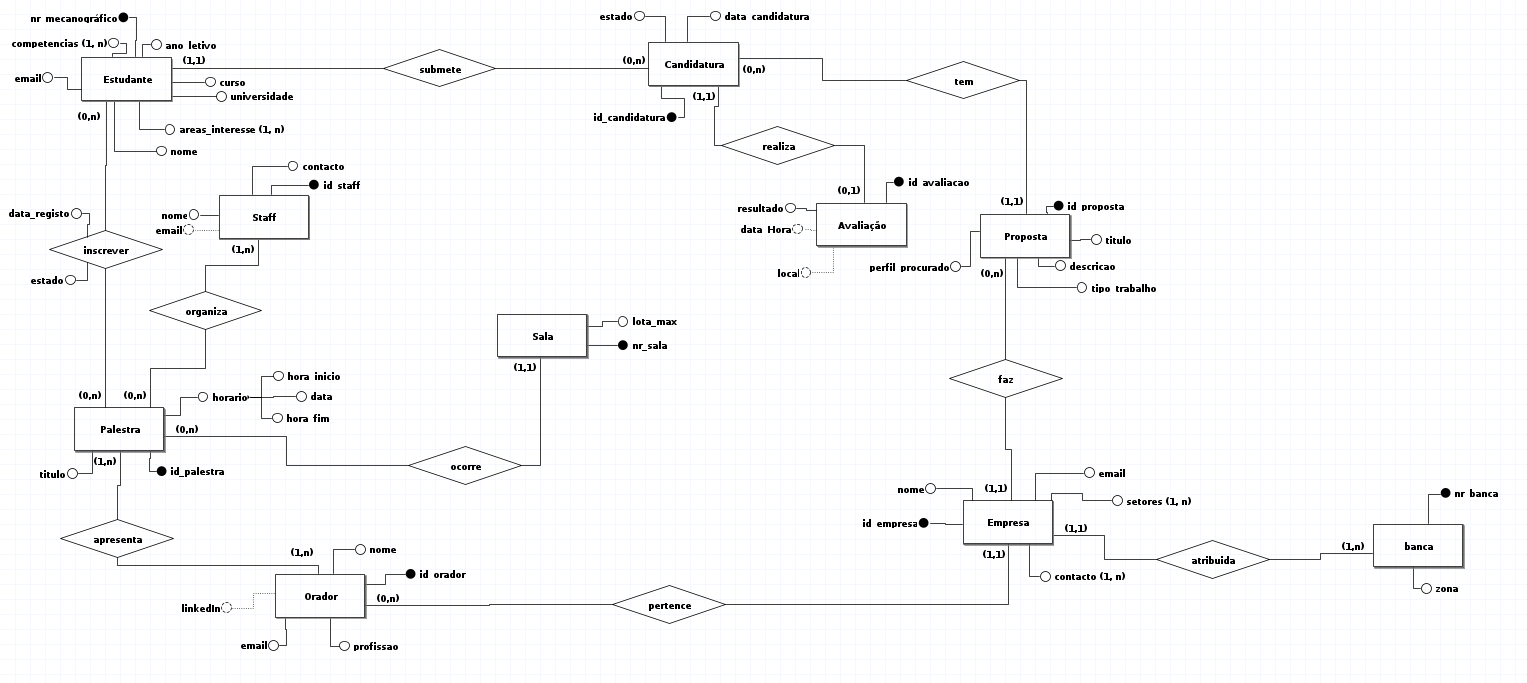
\includegraphics[width=1\textwidth]{images/conceptual.png}
    \caption{Modelo Conceptual}
    \label{fig:exemplo}
\end{figure}

\newpage
\subsection{Identificação e Caracterização das Entidades}

Com os requisitos feitos podemos admitir já quais serão as entidades abordadas no Modelo Conceptual

\begin{table}[H]
    \centering
    
    \label{tab:relacionamentos}
    \begin{tabularx}{\textwidth}{|l|X|l|l|}
        \hline
        \textbf{Designação} & \textbf{Descrição} & \textbf{Sinonimos} & \textbf{Ocorrências} \\
        \hline
        Estudante & \makecell[l]{Pessoa inscrita no evento\\com dados pessoais \\ e académico} & Aluno & Várias \\
        \hline
        Palestra & \makecell[l]{Sessão de apresentação\\de um tema específico} & Apresentação & Várias \\
        \hline
        Staff & \makecell[l]{Equipa de apoio\\responsável pela\\ organização} & Equipa & Várias \\
        \hline
        Orador & \makecell[l]{Pessoa que apresenta\\ou conduz uma palestra} & Palestrante & Várias \\
        \hline
        Empresa & \makecell[l]{Entidade participante\\com banca e propostas} & Parceira & Várias \\
        \hline
        Sala & \makecell[l]{Espaço físico onde\\ decorrem as sessões} & Local & Várias \\
        \hline
        Banca & \makecell[l]{Stand ou espaço de\\exposição da empresa} & Stand & Várias \\
        \hline
        Proposta & \makecell[l]{Oferta de estágio ou\\emprego apresentada} & Oferta & Várias \\
        \hline
        Avaliação & \makecell[l]{Classificação ou feedback\\sobre uma candidatura} & Feedback & Várias \\
        \hline
        Candidatura & \makecell[l]{Pedido de um estudante\\a uma proposta de empresa} & Inscrição & Várias \\
        \hline
        Participante & \makecell[l]{Pessoa envolvida no evento\\(estudante, orador, staff)} & Ator & Várias \\
        \hline
    \end{tabularx}
    \caption{Entidades e sua respetiva descrição.}

\end{table}

\subsection{Identificação e Caracterização dos Relacionamentos}

Dadas as entidades a nossa equipa tem de decidir o comportamento entre elas com os relacionamentos
que nos dão uma visão clara da utilidade da entidade definida:

\begin{table}[H]

\centering
\renewcommand{\arraystretch}{1.2}
\begin{tabularx}{\textwidth}{|X|l|X|l|X|}
\hline
\textbf{Entidade} & \textbf{Mul} & \textbf{Relacionamento}  & \textbf{Mul}  & \textbf{Entidade} \\ \hline

Estudante & 1 & submete & N & Candidatura \\ \hline
Estudante & N & inscrever & M & Palestra \\ \hline
Staff & N & organiza & M & Palestra \\ \hline
Palestra & N & ocorre & 1 & Sala \\ \hline
Orador & M & apresenta & N  & Palestra \\ \hline
Orador & N & pertence & 1 & Empresa \\ \hline
Empresa & 1 & faz & N  & Proposta \\ \hline
Proposta & N & tem & 1  & Candidatura \\ \hline
Candidatura & 1 & realiza & 1  & Avaliação \\ \hline
Empresa & 1 & atribuida & N  & Banca \\ \hline

\end{tabularx}
\caption{Caracterização da tabela lógica da Avaliação.}
\end{table}

\subsection{Identificação e Caracterização dos Atributos das Entidades e dos Relacionamentos}

Após a identificação das entidades e dos relacionamentos principais do domínio,
torna-se necessário detalhar os atributos que caracterizam cada elemento do
modelo. Este ponto apresenta, por isso, um dicionário de dados onde são
definidos os nomes dos atributos, os respetivos tipos, restrições de integridade
e exemplos de valores possíveis. Esta caracterização permite clarificar a
estrutura informacional da base de dados e serve de suporte à passagem do modelo
conceptual para a implementação lógica e física do sistema FENUM.

{
\tiny
\setlength{\extrarowheight}{3pt}
\setlength{\tabcolsep}{3pt}
\begin{longtable}{|>{\raggedright\arraybackslash}p{1.55cm}|>{\raggedright\arraybackslash}p{2.3cm}|>{\raggedright\arraybackslash}p{2.15cm}|>{\raggedright\arraybackslash}p{2.25cm}|>{\raggedright\arraybackslash}p{3.3cm}|>{\raggedright\arraybackslash}p{1.85cm}|}
    
    \hline
    \textbf{Entidade} & \textbf{Atributo} & \textbf{Tipo} & \textbf{Restrições} & \textbf{Descrição} & \textbf{Exemplo} \\
    \hline
    \endfirsthead
    
    % Cabeçalho para as páginas seguintes
    \multicolumn{6}{c}{{\tablename\ \thetable{}, continuação da página anterior}} \\
    \hline
    \textbf{Entidade} & \textbf{Atributo} & \textbf{Tipo} & \textbf{Restrições} & \textbf{Descrição} & \textbf{Exemplo} \\
    \hline
    \endhead
    
    % Rodapé no final de cada página, exceto a última
    \hline
    \multicolumn{6}{r}{\textit{Continua na página seguinte...}} \\
    \endfoot
    
    % Rodapé na última página, onde fica a legenda
    \hline
    \caption{Dicionário de Dados: Caracterização Física dos Atributos}
    \label{tab:dicionario_dados} \\
    \endlastfoot

    % Conteúdo da tabela
    \textbf{Estudante} & nr\_mecanografico & INT & PRIMARY KEY & ID único do aluno atribuído pela instituição. & 100234 \\ 
    \cline{2-6}
     & email & VARCHAR(100) & NOT NULL & Correio eletrónico institucional ou pessoal. & joao@uminho.pt \\
    \cline{2-6}
     & curso & VARCHAR(100) & NOT NULL & Designação do curso que frequenta. & Eng. Informática \\
    \cline{2-6}
     & universidade & ENUM & NOT NULL, DEF 'outro' & Instituição de ensino de origem. & 'Universidade do Minho' \\
    \cline{2-6}
     & nome & VARCHAR(45) & NOT NULL & Nome próprio ou completo do estudante. & João Silva \\
    \cline{2-6}
     & competencias & - & - & \multicolumn{2}{>{\raggedright\arraybackslash}p{5.15cm}|}{\textit{(Mapeado na tabela externa: Competencias)}} \\
    \cline{2-6}
     & areasdeinteresse & - & - & \multicolumn{2}{>{\raggedright\arraybackslash}p{5.15cm}|}{\textit{(Mapeado na tabela externa: AreasdeInteresse)}} \\ 
    \hline
    
    \textbf{Empresa} & idEmpresa & INT & PK, AUTO\_INC & Identificador único interno da empresa. & 1 \\
    \cline{2-6}
     & nome & VARCHAR(45) & NOT NULL & Designação comercial da entidade parceira. & TechCorp Lda \\
    \cline{2-6}
     & email & VARCHAR(100) & NOT NULL & Email institucional para recrutamento. & rh@techcorp.pt \\
    \cline{2-6}
     & setores & - & - & \multicolumn{2}{>{\raggedright\arraybackslash}p{5.15cm}|}{\textit{(Mapeado na tabela externa: Setores)}} \\
    \cline{2-6}
     & contacto & - & - & \multicolumn{2}{>{\raggedright\arraybackslash}p{5.15cm}|}{\textit{(Mapeado na tabela externa: Contacto)}} \\ 
    \hline
    
    \textbf{Staff} & idStaff & INT & PK, AUTO\_INC & ID único do membro da organização. & 5 \\
    \cline{2-6}
     & nome & VARCHAR(45) & NOT NULL & Nome do elemento do staff. & Ana Costa \\
    \cline{2-6}
     & email & VARCHAR(100) & NULL & Email interno para contacto direto. & ana.staff@fenum.pt \\
    \cline{2-6}
     & contacto & VARCHAR(45) & NOT NULL & Número de telemóvel do membro. & 912345678 \\
    \hline
    
    \textbf{Palestra} & idPalestra & INT & PK, AUTO\_INC & Identificador interno da sessão. & 10 \\
    \cline{2-6}
     & titulo & VARCHAR(45) & NOT NULL & Título ou tema abordado na apresentação. & IA no Futuro \\
    \cline{2-6}
     & data\_palestra & DATE & NOT NULL & Data agendada para o evento. & 2026-04-15 \\
    \cline{2-6}
     & hora\_inicio & TIME & NOT NULL & Hora prevista para o arranque da sessão. & 14:30:00 \\
    \cline{2-6}
     & hora\_fim & TIME & NOT NULL & Hora prevista de término. & 15:30:00 \\
    \hline
    
    \textbf{Orador} & idOrador & INT & PK, AUTO\_INC & ID único do palestrante convidado. & 3 \\
    \cline{2-6}
     & nome & VARCHAR(45) & NOT NULL & Nome do orador. & Carlos Mendes \\
    \cline{2-6}
     & profissao & VARCHAR(100) & NOT NULL & Cargo ou função atual. & Data Scientist \\
    \cline{2-6}
     & email & VARCHAR(200) & NOT NULL & Correio eletrónico profissional do orador. & cmendes@corp.pt \\
    \cline{2-6}
     & linkedIn & VARCHAR(45) & NULL & URL ou username do perfil de LinkedIn. & /in/carlosmendes \\
    \hline
    
    \textbf{Sala} & nr\_sala & INT & PRIMARY KEY & Número ou identificação física da sala. & 205 \\
    \cline{2-6}
     & lota\_max & INT & NOT NULL & Capacidade máxima autorizada de pessoas. & 150 \\ 
    \hline
    
    \textbf{Banca} & nr\_banca & INT & PK, AUTO\_INC & Identificador do stand no recinto. & 12 \\
    \cline{2-6}
     & zona & VARCHAR(45) & NOT NULL & Área/Setor do pavilhão onde se encontra. & Zona B - Tech \\ 
    \hline
    
    \textbf{Proposta} & idProposta & INT & PK, AUTO\_INC & Identificador da vaga ou oportunidade. & 45 \\
    \cline{2-6}
     & titulo & VARCHAR(45) & NOT NULL & Nome ou resumo do cargo oferecido. & Estágio Frontend \\
    \cline{2-6}
     & descricao & VARCHAR(200) & NOT NULL & Detalhes das funções e responsabilidades. & Desenho de UIs. \\
    \cline{2-6}
     & tipo\_trabalho & VARCHAR(45) & NOT NULL & Natureza do vínculo oferecido pela empresa. & Estágio de Verão \\
    \cline{2-6}
     & perfil\_procurado & VARCHAR(100) & NOT NULL & Requisitos necessários para se candidatar. & Aluno de 3º ano. \\ 
    \hline

    
    \textbf{Candidatura} & id\_candidatura & INT & PK, AUTO\_INC & Identificador da submissão do aluno. & 128 \\
    \cline{2-6}
     & data\_candidatura & DATE & NOT NULL & Data de entrada do pedido no sistema. & 2026-04-10 \\
    \cline{2-6}
     & estado & ENUM & NOT NULL, DEF 'Em espera' & Situação atual da candidatura. & 'Em espera' \\ 
    \hline
    
    \textbf{Avaliação} & id\_avaliacao & INT & PK, AUTO\_INC & ID do registo de avaliação de entrevista. & 89 \\
    \cline{2-6}
     & resultado & ENUM & NOT NULL, DEF 'A definir' & Parecer final da empresa sobre o candidato. & 'Aceite' \\
    \cline{2-6}
     & local & VARCHAR(45) & NULL & Espaço físico onde ocorreu a entrevista. & Sala 3 - Piso 1 \\
    \cline{2-6}
     & data\_Hora & DATETIME & NULL & Momento em que foi avaliada/entrevistada. & 2026-04-16 10:00:00 \\
\end{longtable}
}

\section{Modelação Lógica}

\subsection{Construção e Validação do Modelo de Dados Lógico}
Com a conclusão e revisão da modelação conceptual, a nossa equipa pôde avançar para a elaboração do Modelo de Dados Lógico, traduzindo as entidades, relacionamentos e restrições previamente definidos para um modelo relacional estruturado.

Nesta fase, recorremos ao \textit{MySQL Workbench} para a criação e organização do esquema da base de dados. A ferramenta permitiu-nos definir tabelas, atributos, chaves primárias e estrangeiras, bem como estabelecer corretamente as relações entre as diferentes entidades. Para além disso, foram aplicadas regras de integridade referencial de forma a garantir a consistência dos dados.

Durante o processo de modelação lógica, tivemos também em consideração a normalização da base de dados, procurando reduzir redundâncias e evitar anomalias de inserção, atualização e eliminação. Assim, as tabelas foram organizadas de acordo com as formas normais mais adequadas ao problema em estudo.

Adicionalmente, o modelo foi validado através da simulação de inserção de dados e testes de integridade, assegurando que todas as restrições definidas eram respeitadas. Esta etapa revelou-se essencial para identificar possíveis inconsistências e otimizar a estrutura antes da implementação final.

Por fim, o \textit{MySQL Workbench} possibilitou ainda a geração automática do script SQL correspondente ao modelo desenvolvido, facilitando a transição para a fase de implementação física da base de dados.


\subsection{Apresentação e Explicação do Modelo Lógico Produzido}

Com base no Modelo Conceptual previamente desenvolvido, a equipa procedeu à construção do Modelo Lógico, efetuando a sua tradução para o paradigma relacional. Durante este processo, foram criadas as tabelas correspondentes a cada entidade identificada, bem como tabelas adicionais sempre que necessário para representar corretamente as relações, em particular nos casos de relações muitos-para-muitos.

Foram igualmente definidos os atributos de cada tabela, as respetivas chaves primárias e estrangeiras, garantindo a integridade referencial entre os diferentes elementos do modelo. A estrutura foi organizada de forma a refletir fielmente as regras de negócio estabelecidas na fase conceptual.


\begin{table}[h]
\textbf{Estudante}

\centering
\renewcommand{\arraystretch}{1.2}
\begin{tabularx}{\textwidth}{|X|l|X|}
\hline
\textbf{Atributo} & \textbf{Tipo de dado} & \textbf{Referência (tabela)} \\ \hline

nr\_mecanográfico & INT & - \\ \hline
Nome & VARCHAR(45) & - \\ \hline
curso & VARCHAR(100) & - \\ \hline
email & VARCHAR(100) & - \\ \hline
universidade & ENUM(...) & - \\ \hline
\end{tabularx}
\caption{Caracterização da tabela lógica do Estudante.}
\end{table}


\begin{table}[h]
\textbf{AreasdeInteresse}

\centering
\renewcommand{\arraystretch}{1.2}
\begin{tabularx}{\textwidth}{|X|l|X|}
\hline
\textbf{Atributo} & \textbf{Tipo de dado} & \textbf{Referência (tabela)} \\ \hline
areasdeinteresse & VARCHAR(200) & - \\ \hline
nr\_mecanográfico & INT & Estudante \\ \hline
\end{tabularx}
\caption{Caracterização da tabela lógica das Areas de Interesse.}
\end{table}


\begin{table}[h]
\textbf{competencias}

\centering
\renewcommand{\arraystretch}{1.2}
\begin{tabularx}{\textwidth}{|X|l|X|}
\hline
\textbf{Atributo} & \textbf{Tipo de dado} & \textbf{Referência (tabela)} \\ \hline

competencias & VARCHAR(200) & - \\ \hline
nr\_mecanográfico & INT & Estudante \\ \hline

\end{tabularx}
\caption{Caracterização da tabela lógica das competencias.}
\end{table}



\begin{table}[h]
\textbf{Inscricao}

\centering
\renewcommand{\arraystretch}{1.2}
\begin{tabularx}{\textwidth}{|X|l|X|}
\hline
\textbf{Atributo} & \textbf{Tipo de dado} & \textbf{Referência (tabela)} \\ \hline

estudante\_nr\_mecanografico & INT & Estudante \\ \hline
palestra\_id\_palestra & INT & Palestra\\ \hline
data\_registo & DATE & - \\ \hline
estado & ENUM(...) & - \\ \hline
\end{tabularx}
\caption{Caracterização da tabela lógica da Inscrição.}
\end{table}

\begin{table}[H]
\textbf{Palestra}

\centering
\renewcommand{\arraystretch}{1.2}
\begin{tabularx}{\textwidth}{|X|l|X|}
\hline
\textbf{Atributo} & \textbf{Tipo de dado} & \textbf{Referência (tabela)} \\ \hline

id\_palestra & INT & - \\ \hline
titulo & VARCHAR(45) & -\\ \hline
data & DATE & - \\ \hline
hora\_inicio & TIME & - \\ \hline
hora\_fim& TIME & - \\ \hline
nr\_sala & INT & Sala \\ \hline
\end{tabularx}
\caption{Caracterização da tabela lógica da Palestra.}
\end{table}

\begin{table}[H]
\textbf{Orador}

\centering
\renewcommand{\arraystretch}{1.2}
\begin{tabularx}{\textwidth}{|X|l|X|}
\hline
\textbf{Atributo} & \textbf{Tipo de dado} & \textbf{Referência (tabela)} \\ \hline

id\_orador & INT & - \\ \hline
nome & VARCHAR(45) & -\\ \hline
profissao & VARCHAR(100) & - \\ \hline
email & VARCHAR(200) & - \\ \hline
linkedIn & VARCHAR(45) & - \\ \hline
empresa\_id\_empresa & INT & Empresa \\ \hline
\end{tabularx}
\caption{Caracterização da tabela lógica do Orador.}
\end{table}

\begin{table}[H]
\textbf{Apresentação}

\centering
\renewcommand{\arraystretch}{1.2}
\begin{tabularx}{\textwidth}{|X|l|X|}
\hline
\textbf{Atributo} & \textbf{Tipo de dado} & \textbf{Referência (tabela)} \\ \hline

orador\_id\_orador & INT & Orador \\ \hline
palestra\_id\_palestra & INT & Palestra\\ \hline

\end{tabularx}
\caption{Caracterização da tabela lógica da apresentação.}
\end{table}

\begin{table}[H]
\textbf{Staff}

\centering
\renewcommand{\arraystretch}{1.2}
\begin{tabularx}{\textwidth}{|X|l|X|}
\hline
\textbf{Atributo} & \textbf{Tipo de dado} & \textbf{Referência (tabela)} \\ \hline

id\_staff & INT & - \\ \hline
nome & VARCHAR(45) & - \\ \hline
email & VARCHAR(100) & - \\ \hline
contacto & VARCHAR(45) & - \\ \hline

\end{tabularx}
\caption{Caracterização da tabela lógica do Staff.}
\end{table}

\begin{table}[H]
\textbf{Organização}

\centering
\renewcommand{\arraystretch}{1.2}
\begin{tabularx}{\textwidth}{|X|l|X|}
\hline
\textbf{Atributo} & \textbf{Tipo de dado} & \textbf{Referência (tabela)} \\ \hline

palestra\_id\_palestra & INT & Palestra \\ \hline
staff\_id\_staff & INT & Staff \\ \hline

\end{tabularx}
\caption{Caracterização da tabela lógica da Organização.}
\end{table}

\begin{table}[H]
\textbf{Sala}

\centering
\renewcommand{\arraystretch}{1.2}
\begin{tabularx}{\textwidth}{|X|l|X|}
\hline
\textbf{Atributo} & \textbf{Tipo de dado} & \textbf{Referência (tabela)} \\ \hline

nr\_sala & INT & - \\ \hline
lota\_max & INT & - \\ \hline

\end{tabularx}
\caption{Caracterização da tabela lógica da Sala.}
\end{table}

\begin{table}[H]
\textbf{Empresa}

\centering
\renewcommand{\arraystretch}{1.2}
\begin{tabularx}{\textwidth}{|X|l|X|}
\hline
\textbf{Atributo} & \textbf{Tipo de dado} & \textbf{Referência (tabela)} \\ \hline

id\_empresa & INT & - \\ \hline
nome & VARCHAR(45) & - \\ \hline
email & VARCHAR(100) & - \\ \hline

\end{tabularx}
\caption{Caracterização da tabela lógica da Empresa.}
\end{table}


\begin{table}[H]
\textbf{Setores}

\centering
\renewcommand{\arraystretch}{1.2}
\begin{tabularx}{\textwidth}{|X|l|X|}
\hline
\textbf{Atributo} & \textbf{Tipo de dado} & \textbf{Referência (tabela)} \\ \hline

setores & VARCHAR(50) & - \\ \hline
empresa\_id\_empresa & INT & Empresa \\ \hline

\end{tabularx}
\caption{Caracterização da tabela lógica dos Setores.}
\end{table}


\begin{table}[H]
\textbf{Contacto}

\centering
\renewcommand{\arraystretch}{1.2}
\begin{tabularx}{\textwidth}{|X|l|X|}
\hline
\textbf{Atributo} & \textbf{Tipo de dado} & \textbf{Referência (tabela)} \\ \hline

contacto & VARCHAR(45) & - \\ \hline
empresa\_id\_empresa & INT & Empresa \\ \hline

\end{tabularx}
\caption{Caracterização da tabela lógica do Contacto.}
\end{table}

\begin{table}[H]
\textbf{Proposta}

\centering
\renewcommand{\arraystretch}{1.2}
\begin{tabularx}{\textwidth}{|X|l|X|}
\hline
\textbf{Atributo} & \textbf{Tipo de dado} & \textbf{Referência (tabela)} \\ \hline

id\_proposta & INT & - \\ \hline
titulo & VARCHAR(45) & - \\ \hline
descricao & VARCHAR(200) & - \\ \hline
tipo\_trabalho & VARCHAR(45) & - \\ \hline
perfil\_procurado & VARCHAR(100) & - \\ \hline
empresa\_id\_empresa & INT & Empresa \\ \hline

\end{tabularx}
\caption{Caracterização da tabela lógica da Proposta.}
\end{table}

\begin{table}[H]
\textbf{Candidatura}

\centering
\renewcommand{\arraystretch}{1.2}
\begin{tabularx}{\textwidth}{|X|l|X|}
\hline
\textbf{Atributo} & \textbf{Tipo de dado} & \textbf{Referência (tabela)} \\ \hline

id\_candidatura & INT & - \\ \hline
data\_candidatura & DATE & - \\ \hline
estado & ENUM(...) & - \\ \hline
proposta\_id\_proposta & INT & Proposta \\ \hline
nr\_mecanografico & INT & Estudante \\ \hline

\end{tabularx}
\caption{Caracterização da tabela lógica da Candidatura.}
\end{table}



\begin{table}[H]
\textbf{Avaliação}

\centering
\renewcommand{\arraystretch}{1.2}
\begin{tabularx}{\textwidth}{|X|l|X|}
\hline
\textbf{Atributo} & \textbf{Tipo de dado} & \textbf{Referência (tabela)} \\ \hline

id\_avaliacao & INT & - \\ \hline
resultado & ENUM(...) & - \\ \hline
local\_av & VARCHAR(45) & - \\ \hline
data\_Hora & DATETIME & - \\ \hline
candidatura\_id\_candidatura & INT & Candidatura \\ \hline

\end{tabularx}
\caption{Caracterização da tabela lógica da Avaliação.}
\end{table}

\begin{table}[H]
\textbf{Banca}

\centering
\renewcommand{\arraystretch}{1.2}
\begin{tabularx}{\textwidth}{|X|l|X|}
\hline
\textbf{Atributo} & \textbf{Tipo de dado} & \textbf{Referência (tabela)} \\ \hline

nr\_banca & INT & - \\ \hline
zona & VARCHAR(45) & - \\ \hline
empresa\_id\_empresa & INT & Empresa \\ \hline

\end{tabularx}
\caption{Caracterização da tabela lógica da Banca.}
\end{table}


\newpage
Apresenta-se de seguida o diagrama do modelo lógico, o qual ilustra de forma estruturada a organização das entidades, os seus respetivos atributos e as relações existentes entre elas, permitindo uma melhor compreensão da forma como a informação é representada e interligada no sistema.
\begin{figure}[h]
    \centering
    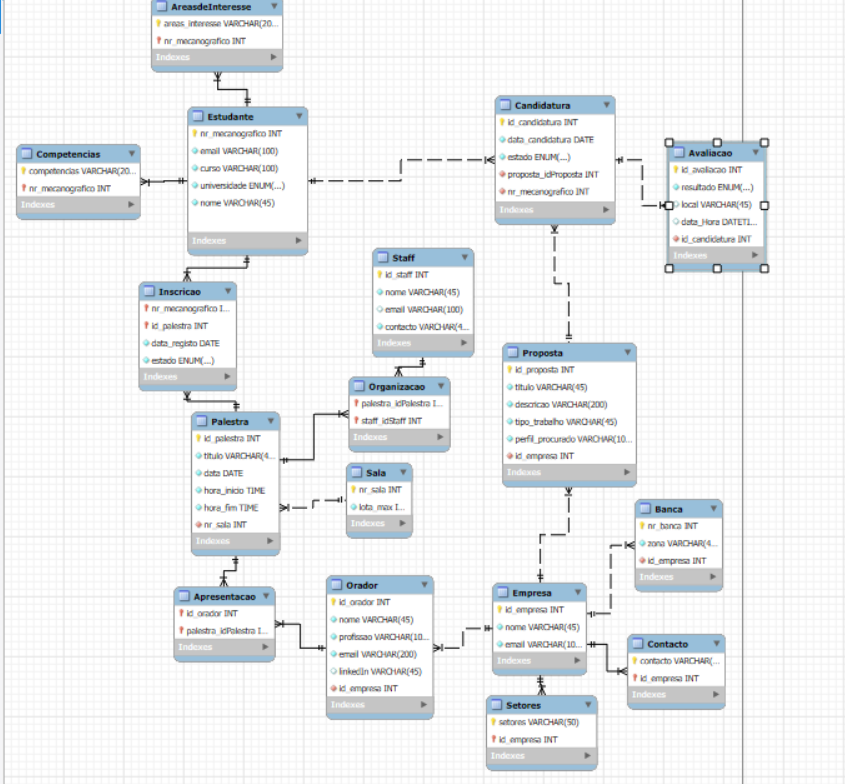
\includegraphics[width=1\textwidth]{images/modelo_logico.png}
    \caption{Modelo Lógico}
    \label{fig:modelo_logico}
\end{figure}



\subsection{Normalização de Dados}

O modelo de dados desenvolvido foi submetido a um processo de normalização
rigoroso, visando a eliminação de redundâncias e a preservação da integridade
referencial. A estrutura apresentada cumpre os requisitos das três primeiras
formas normais (1FN, 2FN e 3FN), conforme detalhado a seguir:


Uma relação encontra-se na 1FN quando todos os seus atributos contêm apenas
valores atómicos e não existem grupos repetitivos. No esquema proposto, este
requisito é garantido através da decomposição de atributos multivalorados em
entidades independentes. 

Exemplos claros desta aplicação são as tabelas \texttt{competencias},
\texttt{AreasdeInteresse} e \texttt{Setores}. Em vez de armazenar múltiplas
competências num único campo de texto na tabela \texttt{Estudante}, cada
competência é registada como uma linha individual vinculada ao
\texttt{nr\_mecanografico} do aluno. Isto assegura a atomicidade exigida pela
1FN, facilitando pesquisas e indexação de dados.


Para atingir a 2FN, a tabela deve estar na 1FN e todos os atributos não-chave
devem possuir uma dependência funcional total da chave primária. Isto é
fundamental em tabelas com chaves compostas para evitar dependências parciais.

No diagrama, as tabelas associativas como \texttt{Inscricao} e
\texttt{Apresentacao} exemplificam este princípio. Na tabela \texttt{Inscricao},
os atributos \texttt{data\_registo} e \texttt{estado} dependem da combinação
única de \texttt{estudante\_nr\_mecanografico} e \texttt{palestra\_idPalestra}.
Não existem atributos que dependam apenas de uma parte da chave composta,
garantindo que a informação sobre a inscrição seja específica à relação entre o
aluno e o evento, respeitando a 2FN.


A 3FN exige que a relação esteja na 2FN e que não existam dependências
transitivas, ou seja, nenhum atributo não-chave deve depender de outro atributo
não-chave.

Esta regra é observada na separação entre as entidades de negócio e os seus
detalhes descritivos. Por exemplo, na tabela \texttt{Proposta}, armazena-se
apenas a chave estrangeira \texttt{empresa\_idEmpresa}. Detalhes como o nome,
email ou contactos da empresa não são replicados na tabela de propostas, mas sim
mantidos exclusivamente na tabela \texttt{Empresa} (ou nas suas tabelas de apoio
como \texttt{Contacto}). Esta estrutura garante que qualquer alteração nos dados
da empresa seja refletida em todo o sistema através de uma única atualização,
eliminando o risco de inconsistências e cumprindo rigorosamente a 3FN.

A aplicação destas normas resulta num esquema relacional robusto e otimizado. A
separação lógica das entidades minimiza o desperdício de espaço e assegura que
as operações de inserção, atualização e deleção não gerem anomalias no sistema
de gestão do evento.

\subsection{Validação do Modelo com Interrogações do Utilizador}

Para confirmar que o modelo lógico desenvolvido é capaz de responder às
necessidades de informação definidas, procedeu-se à expressão de um conjunto
de requisitos de manipulação em álgebra relacional. Este exercício permite
verificar, de forma formal, que as entidades e relações do modelo contêm os
atributos necessários para satisfazer cada interrogação.


\medskip
\noindent\textbf{RM02: Estudantes sem candidaturas}

\noindent Identificar os estudantes que não submeteram qualquer candidatura
corresponde a uma diferença entre o conjunto total de estudantes e o conjunto
dos que têm pelo menos uma candidatura registada:

\[
\pi_{\textit{nr\_mec},\, \textit{nome},\, \textit{curso},\, \textit{universidade}}(\textit{Estudante})
\;-\;
\pi_{\textit{nr\_mec},\, \textit{nome},\, \textit{curso},\, \textit{universidade}}
\bigl(\textit{Estudante} \bowtie \textit{Candidatura}\bigr)
\]

\medskip
\noindent\textbf{RM06: Consulta da banca atribuída a uma empresa}

\noindent Obter a banca e respetiva zona para uma empresa específica requer uma
seleção seguida de uma junção natural entre \textit{Empresa} e \textit{Banca},
projetando apenas os atributos relevantes:

\[
\pi_{\textit{nome},\, \textit{nr\_banca},\, \textit{zona}}
\bigl(\sigma_{\textit{id\_empresa}\,=\,x}(\textit{Empresa} \bowtie \textit{Banca})\bigr)
\]

\medskip
\noindent\textbf{RM07: Palestras da agenda diária de um estudante}

\noindent A componente de palestras da agenda diária de um estudante é obtida
filtrando as inscrições aceites para um estudante e data específicos, com junção
às tabelas \textit{Palestra} e \textit{Sala}:

\[
\pi_{\textit{hora\_inicio},\, \textit{titulo},\, \textit{nr\_sala}}
\Bigl(
  \sigma_{\substack{\textit{nr\_mec}=x \;\land\\ \textit{data}=d \;\land\\ \textit{estado}=\text{`Aceite'}}}
  (\textit{Inscricao} \bowtie \textit{Palestra} \bowtie \textit{Sala})
\Bigr)
\]

\medskip
\noindent\textbf{RM10: Empresas com propostas sem candidaturas}

\noindent Este requisito é resolvido em duas etapas: primeiro isola-se o
conjunto de propostas que não receberam candidaturas através de uma diferença
de conjuntos; depois junta-se o resultado às entidades \textit{Proposta} e
\textit{Empresa} para obter a informação da empresa responsável:

\[
P_{sc} \leftarrow \pi_{\textit{id\_proposta}}(\textit{Proposta})
\;-\;
\pi_{\textit{proposta\_idProposta}}(\textit{Candidatura})
\]
\[
\pi_{\textit{id\_empresa},\, \textit{nome},\, \textit{email}}
\bigl(\textit{Empresa} \bowtie (\textit{Proposta} \bowtie P_{sc})\bigr)
\]


\section{Implementação Física}

Neste capítulo, descreve-se a materialização do modelo lógico no Sistema de Gestão de Bases de Dados escolhido, detalhando as decisões de otimização, segurança e programabilidade.

\subsection{Apresentação e explicação da base de dados implementada}

De forma a iniciar o desenvolvimento do sistema de gestão de base de dados para o evento FENUM, procedeu-se à implementação em \texttt{MySQL} de cada tabela detalhada anteriormente na fase de modelação lógica. Este processo é fundamental para materializar as regras de negócio e garantir que a estrutura de dados suporta todas as funcionalidades previstas.

O processo de implementação física é inaugurado com duas instruções SQL essenciais: a primeira cria a base de dados com o nome "FENUM", e a segunda instrui o SGBD a utilizar este esquema para todas as operações de criação e manipulação que se seguem:

\begin{lstlisting}[language=SQL, caption={Instruções iniciais de criação da base de dados}, label={lst:create_db}]
CREATE DATABASE IF NOT EXISTS FENUM;
USE FENUM;
\end{lstlisting}

A estrutura da base de dados foi construída seguindo uma ordem de precedência que respeita as dependências de integridade referencial, assegurando que as tabelas "mestre" sejam criadas antes das tabelas que as referenciam através de chaves estrangeiras.

\subsubsection*{Estrutura de Entidades e Atributos}

As tabelas foram configuradas utilizando tipos de dados otimizados para o volume de informação esperado:

\begin{itemize}
    \item \textbf{Identificadores:} Utilizou-se o tipo \texttt{INT} com a propriedade \texttt{AUTO\_INCREMENT} para chaves primárias artificiais, e \texttt{INT} simples para chaves naturais como o número mecanográfico do \textit{Estudante}.
    \item \textbf{Domínios Restritos:} Para colunas que admitem apenas um conjunto fixo de valores, como o estado de uma \textit{Candidatura} ou a universidade de origem, aplicou-se o tipo \texttt{ENUM}. Esta escolha permite uma validação automática ao nível do SGBD e uma gestão eficiente de espaço.
    \item \textbf{Integridade Semântica:} Foram aplicadas restrições \texttt{NOT NULL} em campos críticos e cláusulas \texttt{CHECK} (por exemplo, na lotação máxima da \textit{Sala}) para impedir a inserção de dados inconsistentes.
\end{itemize}


\subsubsection*{Relacionamentos e Integridade Referencial}

A implementação física reflete fielmente as cardinalidades do modelo lógico através do uso sistemático de chaves estrangeiras (\textit{FOREIGN KEY}). Relacionamentos de muitos-para-muitos, como as competências de um estudante ou as inscrições em palestras, foram materializados através de tabelas de ligação (\textit{Competencias}, \textit{Inscricao}), garantindo a rastreabilidade total da informação no sistema.

\begin{lstlisting}[language=SQL, caption={Criação de uma tabela de relação N:M}, label={lst:create_db}]
CREATE TABLE Candidatura(
	id_candidatura INT AUTO_INCREMENT PRIMARY KEY,
    data_candidatura DATE NOT NULL,
    estado ENUM('Em espera', 'Aceite', 'Recusada')
		NOT NULL DEFAULT 'Em espera',
	proposta_idProposta INT NOT NULL,
    nr_mecanografico INT NOT NULL,
	FOREIGN KEY (proposta_idProposta) REFERENCES Proposta(id_proposta),
    FOREIGN KEY (nr_mecanografico) REFERENCES Estudante(nr_mecanografico)
);
\end{lstlisting}

Ao adotar esta abordagem rigorosa na implementação física, assegura-se que a
base de dados FENUM é não apenas um repositório de dados, mas um sistema íntegro
e preparado para a fase de povoamento e exploração de dados.

\subsection{Criação de utilizadores da base de dados}

A segurança e a integridade da base de dados FENUM foram asseguradas através da
implementação de um modelo de controlo de acessos baseado em papéis
(\textit{Role-Based Access Control} - RBAC). Esta estratégia permite uma gestão
centralizada e eficiente das permissões, garantindo que cada interveniente no
ecossistema FENUM, desde a equipa de \textit{staff} até aos estudantes e
empresas parceiras, tenha acesso apenas aos dados e operações estritamente
necessários para o desempenho das suas funções, cumprindo o requisito de
segurança US-RC01.

Foram definidos três papéis distintos, aos quais foram atribuídos privilégios
específicos:

\begin{itemize}
    \item \textbf{Staff:} Detém controlo total sobre o esquema, sendo
    responsável pela gestão administrativa, manutenção e configuração de bancas
    e infraestrutura.
    \item \textbf{Empresa:} Acesso limitado através de \textit{Views},
    permitindo apenas a consulta de candidatos associados às suas ofertas e o
    mapa de bancas, protegendo a privacidade dos estudantes.
    \item \textbf{Estudante:} Acesso restrito para consulta de propostas,
    palestras, inscrições e candidaturas próprias, com permissão de inserção
    em registos de candidaturas e inscrições.
\end{itemize}

O procedimento de criação de utilizadores e atribuição de permissões foi
executado conforme ilustrado no código SQL seguinte:

\begin{lstlisting}[language=SQL, caption={Configuração de Roles e Utilizadores}, label={lst:roles}]
-- Criacao das Roles
CREATE ROLE 'staff';
CREATE ROLE 'empresa';
CREATE ROLE 'estudante';

-- Atribuicao de privilegios (Exemplos)
GRANT ALL PRIVILEGES ON FENUM.* TO 'staff';
GRANT SELECT ON FENUM.v_candidatos_por_empresa TO 'empresa';
GRANT SELECT ON FENUM.Inscricao TO 'estudante';
GRANT INSERT ON FENUM.Inscricao TO 'estudante';

-- Criacao de utilizadores e associacao as Roles
CREATE USER 'organizacao'@'localhost' IDENTIFIED BY 'fenum_org_2026';
GRANT 'staff' TO 'organizacao'@'localhost';
\end{lstlisting}



Esta configuração garante que qualquer tentativa de acesso não autorizado seja
bloqueada ao nível do SGBD, mitigando riscos de corrupção ou exfiltração de
dados sensíveis. A utilização de credenciais específicas para cada perfil
reforça a rastreabilidade das operações realizadas por cada entidade no sistema.

\begin{lstlisting}[language=SQL, caption={exemplo de utilização das permissões}, label={lst:roles}]
SHOW GRANTS FOR 'estudante';
\end{lstlisting}

\subsection{Povoamento da base de dados}

O processo de povoamento da base de dados FENUM não se resumiu à mera inserção
de registos, mas constituiu uma etapa crítica de validação e teste de estresse
da estrutura implementada. O objetivo primordial desta fase foi assegurar que o
esquema SQL (restrições de domínio, chaves primárias e estrangeiras) e as regras
de negócio embutidas (\textit{Triggers}) operam em perfeita sintonia.

\subsubsection*{Metodologia de Carga}
Para garantir a consistência dos dados, a ordem de povoamento foi definida
seguindo um critério de dependência hierárquica (ordem topológica). Procedeu-se
à inserção das entidades independentes (tabelas mestre) previamente à inserção
nas tabelas dependentes. Este rigor foi essencial para evitar violações de
integridade referencial, garantindo que qualquer \textit{Foreign Key} inserida
tivesse uma contrapartida válida na tabela de origem.

Adicionalmente, a carga foi concebida para ser:
\begin{itemize}[leftmargin=1.5cm]
    \item \textbf{Repetível:} possibilidade de recriar o estado inicial de testes de forma determinística;
    \item \textbf{Auditável:} sequência lógica de operações claramente identificável no script;
    \item \textbf{Extensível:} preparada para aumento de volume de dados sem alterar a estratégia de execução.
\end{itemize}

\subsubsection*{Cenários de Validação}
O conjunto de dados escolhido foi desenhado para simular o comportamento de um evento real, abrangendo cenários de teste específicos:
\begin{itemize}[leftmargin=1.5cm]
    \item \textbf{Integridade Referencial:} verificação de que a inserção de um aluno sem universidade válida ou numa banca inexistente resulta num erro de \textit{rollback} pelo SGBD.
    \item \textbf{Restrições de Domínio:} testes com valores de \texttt{ENUM} (ex: estados de candidatura) e restrições \texttt{CHECK} (ex: lotações de sala > 0).
    \item \textbf{Lógica Procedimental:} validação dos \textit{Triggers} de negócio. Por exemplo, ao inserir uma inscrição numa palestra cuja lotação foi atingida pelo povoamento, verificou-se se o estado da inscrição foi automaticamente definido como 'Recusado'.
\end{itemize}

O script de povoamento, cuja estrutura principal é apresentada na
Listagem~\ref{lst:povoar}, foi concebido de forma a ser executável na íntegra,
estabelecendo o estado de repouso da base de dados para as fases de exploração e
consulta.

\lstinputlisting[language=SQL, inputencoding=utf8/latin1, caption={Excerto do script de povoamento (\texttt{povoar.sql})}, label={lst:povoar}]{../modelo/povoar.sql}

\begin{figure}[h]
    \centering
    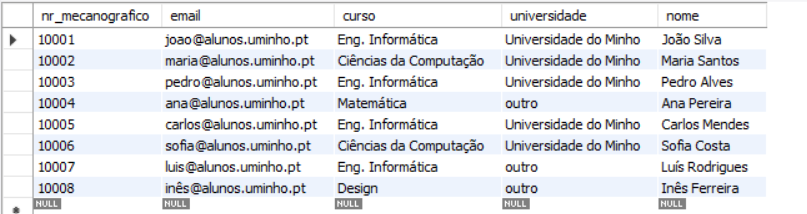
\includegraphics[width=1\textwidth]{images/povoamento.png}
    \caption{Resultado das tabelas com o povoamento}
    \label{fig:povoamento}
\end{figure}

\subsubsection*{Verificação Pós-carga e Critérios de Aceitação}
Após a execução integral do povoamento, foi realizada uma validação técnica com foco em três níveis:
\begin{itemize}[leftmargin=1.5cm]
    \item \textbf{Completude:} confirmação de existência de dados nas entidades nucleares (Estudante, Empresa, Proposta, Candidatura, Palestra);
    \item \textbf{Coerência Relacional:} verificação de correspondência entre chaves primárias e chaves estrangeiras em tabelas de associação;
    \item \textbf{Conformidade de Negócio:} validação de estados, lotações e resultados processados por regras automáticas do sistema.
\end{itemize}

A confirmação da integridade após a carga dos dados, realizada através de consultas de contagem e inspeção de chaves estrangeiras, permitiu validar que a arquitetura FENUM está preparada para a exploração de dados complexos com total confiança na precisão da informação.

\subsection{Cálculo do espaço da base de dados (inicial e taxa de crescimento anual)}

É preciso perceber o espaço que a base de dados poderá vir a ocupar, pra isso nossa equipe
fará uma estimativa de espaço necessário para armazenar toda a informação contida 
na base de dados. Também estimaremos o crescimento do evento para os proximos anos com o aumento
natural de alunos na Universidade do Minho. 

Representaremos o tamanho de cada tipos de dados usados no nosso sistema na seguinte tabela
com referência no Manual SQL 9.7:

\begin{table}[H]

\centering
\renewcommand{\arraystretch}{1.2}
\begin{tabular}{|c|c|}
\hline
\textbf{Tipos de Dados} & \textbf{Tamanho (em bytes)}  \\ \hline

INT & 4  \\ \hline
DATE & 3  \\ \hline
VARCHAR(N) & N+1  \\ \hline
ENUM('valor1',...) & 1 ou 2 \\ \hline
DATETIME & 8 \\ \hline
\end{tabular}
\caption{Tipos de dados utilizados utilizados e o seu tamanho (bytes)}
\end{table}

Por cada cada tabela estimamos a soma dos tamanhos utilizados com os tipos de dados e os 
seus respetivos tamanho:

\begin{table}[H]
\centering
\renewcommand{\arraystretch}{1.2}
\begin{tabular}{|c|c|c|c|}
\hline
\textbf{Tabela} & \textbf{Nome da Coluna} & \textbf{Tipo de Dado} & \textbf{Tamanho} \\ \hline
Estudante & "nr\_mecanografico" & INT & 4 \\ \hline
"& "email" & VARCHAR(100) & 101 \\ \hline
"& "curso" & VARCHAR(100) & 101 \\ \hline
"& "universidade" & ENUM(...) & 2 \\ \hline
"& "nome" & VARCHAR(45) & 46 \\ \hline
- & - & - & - \\ \hline
\textbf{Soma:} & - & - & 254 \\ \hline 
\end{tabular}

\caption{Espaço ocupado pela tabela Estudante pra cada registo}
\end{table}

\begin{table}[H]
\centering
\renewcommand{\arraystretch}{1.2}
\begin{tabular}{|c|c|c|c|}
\hline
\textbf{Tabela} & \textbf{Nome da Coluna} & \textbf{Tipo de Dado} & \textbf{Tamanho} \\ \hline
Competencias & "competencias" & VARCHAR(200) & 201 \\ \hline
"& "nr\_mecanografico" & INT & 4 \\ \hline
- & - & - & - \\ \hline
\textbf{Soma:} & - & - & 205 \\ \hline
\end{tabular}

\caption{Espaço ocupado pela tabela Competencias por registo}
\end{table}

\begin{table}[H]
\centering
\renewcommand{\arraystretch}{1.2}
\begin{tabular}{|c|c|c|c|}
\hline
\textbf{Tabela} & \textbf{Nome da Coluna} & \textbf{Tipo de Dado} & \textbf{Tamanho} \\ \hline
AreasdeInteresse & areas\_interesse & VARCHAR(200) & 201 \\ \hline
"&  "nr\_mecanografico" & INT & 4 \\ \hline
- & - & - & - \\ \hline
\textbf{Soma:} & - & - & 205 \\ \hline
\end{tabular}

\caption{Espaço ocupado pela tabela AreasdeInteresse por registo}
\end{table}

\begin{table}[H]
\centering
\renewcommand{\arraystretch}{1.2}
\begin{tabular}{|c|c|c|c|}
\hline
\textbf{Tabela} & \textbf{Nome da Coluna} & \textbf{Tipo de Dado} & \textbf{Tamanho} \\ \hline
Candidatura & "id\_candidatura" & INT & 4 \\ \hline
"& "data\_candidatura" & DATE & 3 \\ \hline
"& "estado" & ENUM(...) & 1 \\ \hline
"& "proposta\_idProposta" & INT & 4 \\ \hline
"& "nr\_mecanografico" & INT & 4 \\ \hline
- & - & - & - \\ \hline
\textbf{Soma:} & - & - & 19 \\ \hline
\end{tabular}

\caption{Espaço ocupado pela tabela Candidatura por registo}
\end{table}

\begin{table}[H]
\centering
\renewcommand{\arraystretch}{1.2}
\begin{tabular}{|c|c|c|c|}
\hline
\textbf{Tabela} & \textbf{Coluna} & \textbf{Tipo} & \textbf{Tamanho} \\ \hline
Avaliacao & id\_avaliacao & INT & 4 \\ \hline
& resultado & ENUM & 1 \\ \hline
& local & VARCHAR(45) & 46 \\ \hline
& data\_Hora & DATETIME & 8 \\ \hline
& id\_candidatura & INT & 4 \\ \hline
\textbf{Soma} & & & \textbf{63} \\ \hline
\end{tabular}
\caption{Espaço por registo da tabela Avaliacao}
\end{table}

\begin{table}[H]
\centering
\renewcommand{\arraystretch}{1.2}
\begin{tabular}{|c|c|c|c|}
\hline
\textbf{Tabela} & \textbf{Coluna} & \textbf{Tipo} & \textbf{Tamanho} \\ \hline
Proposta & id\_proposta & INT & 4 \\ \hline
& titulo & VARCHAR(45) & 46 \\ \hline
& descricao & VARCHAR(200) & 201 \\ \hline
& tipo\_trabalho & VARCHAR(45) & 46 \\ \hline
& perfil\_procurado & VARCHAR(100) & 101 \\ \hline
& id\_empresa & INT & 4 \\ \hline
\textbf{Soma} & & & \textbf{402} \\ \hline
\end{tabular}
\caption{Espaço por registo da tabela Proposta}
\end{table}

\begin{table}[H]
\centering
\renewcommand{\arraystretch}{1.2}
\begin{tabular}{|c|c|c|c|}
\hline
\textbf{Tabela} & \textbf{Coluna} & \textbf{Tipo} & \textbf{Tamanho} \\ \hline
Empresa & id\_empresa & INT & 4 \\ \hline
& nome & VARCHAR(45) & 46 \\ \hline
& email & VARCHAR(100) & 101 \\ \hline
\textbf{Soma} & & & \textbf{151} \\ \hline
\end{tabular}
\caption{Espaço por registo da tabela Empresa}
\end{table}


\begin{table}[H]
\centering
\renewcommand{\arraystretch}{1.2}
\begin{tabular}{|c|c|c|c|}
\hline
\textbf{Tabela} & \textbf{Coluna} & \textbf{Tipo} & \textbf{Tamanho} \\ \hline
Palestra & id\_palestra & INT & 4 \\ \hline
& titulo & VARCHAR(45) & 46 \\ \hline
& data & DATE & 3 \\ \hline
& hora\_inicio & TIME & 3 \\ \hline
& hora\_fim & TIME & 3 \\ \hline
& nr\_sala & INT & 4 \\ \hline
\textbf{Soma} & & & \textbf{63} \\ \hline
\end{tabular}
\caption{Espaço por registo da tabela Palestra}
\end{table}

\begin{table}[H]
\centering
\renewcommand{\arraystretch}{1.2}
\begin{tabular}{|c|c|c|c|}
\hline
\textbf{Tabela} & \textbf{Coluna} & \textbf{Tipo} & \textbf{Tamanho} \\ \hline
Inscricao & nr\_mecanografico & INT & 4 \\ \hline
& id\_palestra & INT & 4 \\ \hline
& data\_registo & DATE & 3 \\ \hline
& estado & ENUM & 1 \\ \hline
\textbf{Soma} & & & \textbf{12} \\ \hline
\end{tabular}
\caption{Espaço por registo da tabela Inscricao}
\end{table}

\begin{table}[H]
\centering
\renewcommand{\arraystretch}{1.2}
\begin{tabular}{|c|c|c|c|}
\hline
\textbf{Tabela} & \textbf{Coluna} & \textbf{Tipo} & \textbf{Tamanho} \\ \hline
Sala & nr\_sala & INT & 4 \\ \hline
& lota\_max & INT & 4 \\ \hline
\textbf{Soma} & & & \textbf{8} \\ \hline
\end{tabular}
\caption{Espaço por registo da tabela Sala}
\end{table}


\begin{table}[H]
\centering
\renewcommand{\arraystretch}{1.2}
\begin{tabular}{|c|c|c|c|}
\hline
\textbf{Tabela} & \textbf{Coluna} & \textbf{Tipo} & \textbf{Tamanho} \\ \hline
Organizacao & id\_palestra & INT & 4 \\ \hline
& staff\_idStaff & INT & 4 \\ \hline
\textbf{Soma} & & & \textbf{8} \\ \hline
\end{tabular}
\caption{Espaço por registo da tabela Organizacao}
\end{table}

\begin{table}[H]
\centering
\renewcommand{\arraystretch}{1.2}
\begin{tabular}{|c|c|c|c|}
\hline
\textbf{Tabela} & \textbf{Coluna} & \textbf{Tipo} & \textbf{Tamanho} \\ \hline
Staff & id\_staff & INT & 4 \\ \hline
& nome & VARCHAR(45) & 46 \\ \hline
& email & VARCHAR(100) & 101 \\ \hline
& contacto & VARCHAR(45) & 46 \\ \hline
\textbf{Soma} & & & \textbf{197} \\ \hline
\end{tabular}
\caption{Espaço por registo da tabela Staff}
\end{table}

\begin{table}[H]
\centering
\renewcommand{\arraystretch}{1.2}
\begin{tabular}{|c|c|c|c|}
\hline
\textbf{Tabela} & \textbf{Coluna} & \textbf{Tipo} & \textbf{Tamanho} \\ \hline
Orador & id\_orador & INT & 4 \\ \hline
& nome & VARCHAR(45) & 46 \\ \hline
& profissao & VARCHAR(45) & 46 \\ \hline
& email & VARCHAR(200) & 201 \\ \hline
& linkedIn & VARCHAR(45) & 46 \\ \hline
& id\_empresa & INT & 4 \\ \hline
\textbf{Soma} & & & \textbf{347} \\ \hline
\end{tabular}
\caption{Espaço por registo da tabela Orador}
\end{table}


\begin{table}[H]
\centering
\renewcommand{\arraystretch}{1.2}
\begin{tabular}{|c|c|c|c|}
\hline
\textbf{Tabela} & \textbf{Coluna} & \textbf{Tipo} & \textbf{Tamanho} \\ \hline
Contacto & contacto & VARCHAR(45) & 46 \\ \hline
& id\_empresa & INT & 4 \\ \hline
\textbf{Soma} & & & \textbf{50} \\ \hline
\end{tabular}
\caption{Espaço por registo da tabela Contacto}
\end{table}

\begin{table}[H]
\centering
\renewcommand{\arraystretch}{1.2}
\begin{tabular}{|c|c|c|c|}
\hline
\textbf{Tabela} & \textbf{Coluna} & \textbf{Tipo} & \textbf{Tamanho} \\ \hline
Setores & setores & VARCHAR(50) & 51 \\ \hline
& id\_empresa & INT & 4 \\ \hline
\textbf{Soma} & & & \textbf{55} \\ \hline
\end{tabular}
\caption{Espaço por registo da tabela Setores}
\end{table}

\begin{table}[H]
\centering
\renewcommand{\arraystretch}{1.2}
\begin{tabular}{|c|c|c|c|}
\hline
\textbf{Tabela} & \textbf{Coluna} & \textbf{Tipo} & \textbf{Tamanho} \\ \hline
Banca & nr\_banca & INT & 4 \\ \hline
& zona & VARCHAR(45) & 46 \\ \hline
& id\_empresa & INT & 4 \\ \hline
\textbf{Soma} & & & \textbf{54} \\ \hline
\end{tabular}
\caption{Espaço por registo da tabela Banca}
\end{table}

\begin{table}[H]
\centering
\renewcommand{\arraystretch}{1.2}
\begin{tabular}{|c|c|c|c|}
\hline
\textbf{Tabela} & \textbf{Coluna} & \textbf{Tipo} & \textbf{Tamanho} \\ \hline
Apresentacao & id\_orador & INT & 4 \\ \hline
& palestra\_idPalestra & INT & 4 \\ \hline
\textbf{Soma} & & & \textbf{8} \\ \hline
\end{tabular}
\caption{Espaço por registo da tabela Apresentacao}
\end{table}

Num evento do tipo feira de emprego, como o organizado na Universidade do Minho,
é expectável a participação de um número elevado de estudantes e empresas, bem
como a ocorrência de várias interações entre os diferentes intervenientes.
Assim, torna-se relevante estimar o número de registos que serão armazenados na
base de dados, de forma a avaliar o espaço necessário.

Considerando um cenário realista, admite-se a participação de aproximadamente
3000 estudantes, provenientes de diferentes cursos e anos curriculares. Cada
estudante poderá submeter, em média, 3 candidaturas, originando cerca de 9000
registos na tabela Candidatura.

Relativamente às empresas, estima-se a presença de cerca de 100 empresas, cada
uma com uma média de 5 propostas de trabalho, o que resulta em aproximadamente
500 registos na tabela Proposta. Cada empresa poderá ainda possuir múltiplos
contactos e áreas de atuação, levando a cerca de 200 registos na tabela Contacto
e 150 registos na tabela Setores.

No que diz respeito às avaliações, assumindo que uma parte significativa das
candidaturas evolui para entrevistas, estima-se que cerca de 50\% das
candidaturas resultem em avaliações, correspondendo a aproximadamente 4500
registos na tabela Avaliacao.

Para atividades paralelas, como palestras, admite-se a existência de cerca de 20
palestras, com uma média de 150 inscrições cada, resultando em cerca de 2500
registos na tabela Inscricao. Estas palestras poderão envolver aproximadamente
30 oradores, originando também registos nas tabelas Orador e Apresentacao.

Adicionalmente, cada estudante poderá ter em média 15 competências e 1,5 áreas de
interesse, originando cerca de 45000 registos na tabela Competencias e 4500
registos na tabela AreasdeInteresse.

\begin{table}[H]
\centering
\renewcommand{\arraystretch}{1.2}
\begin{tabular}{|c|c|c|c|}
\hline
\textbf{Tabela} & \textbf{Quantidade de registos (estimado)} & \textbf{Tamanho (bytes)}\\ \hline
Estudante & 3000 &  762000 \\ \hline
Competencias & 45000 & 922500 \\ \hline
AreasdeInteresse & 4500 & 922500 \\ \hline
Candidatura & 9000 & 171000 \\ \hline
Avaliacao & 4500 & 283500\\ \hline
Proposta & 500 & 201000 \\ \hline
Empresa & 100 & 15100\\ \hline
Palestra & 20 & 1260\\ \hline
Inscricao & 2500 & 30000\\ \hline
Sala & 20 & 160 \\ \hline
Organizacao & 60 & 480\\ \hline
Staff & 30 & 5910\\ \hline
Orador & 30 & 10410\\ \hline
Contacto & 200 & 10000\\ \hline
Setores & 150 & 8250\\ \hline
Banca & 100 & 5400\\ \hline
Apresentacao & 30 & 240\\ \hline
\textbf{Soma}& - &  3322710\\ \hline

\end{tabular}
\caption{Tamanho estimado da base de dados}
\end{table}

No fim temos uma estimativa de 3322710 bytes ou 3.32 MB. Esta estimativa permite
concluir que o sistema deverá suportar dezenas de milhares de registos, sendo as
tabelas relacionadas com os estudantes (como Competencias, Candidatura e
AreasdeInteresse) as que apresentam maior volume de dados, influenciando
significativamente o espaço total necessário para armazenamento.

\subsection{Definição e caracterização de vistas de utilização em SQL}

A implementação de vistas assume um papel fundamental na base de dados da FENUM,
tendo em conta a diversidade de intervenientes envolvidos no evento,
nomeadamente empresas, estudantes e elementos do staff. Estas vistas permitem
apresentar a informação de forma organizada e adaptada às necessidades
específicas de cada tipo de utilizador, facilitando o acesso aos dados
relevantes e promovendo uma maior eficiência na sua utilização.


A vista v\_candidatos\_por\_empresa permite consultar todas as candidaturas
realizadas, apresentando informação relevante como o estado da candidatura, a
data, a proposta associada, o nome do candidato e a empresa responsável pela
proposta. Esta vista facilita a análise das candidaturas por empresa e por
proposta.

\begin{lstlisting}[language=SQL,caption={Vista que demonstra as empresas e os candidatos com a sua proposta}, label={lst:roles}]
CREATE VIEW v_candidatos_por_empresa AS
SELECT
    c.id_candidatura,
    c.estado,
    c.data_candidatura,
    p.titulo AS proposta,
    est.nome AS candidato,
    e.nome AS Empresa
FROM Candidatura c
JOIN Proposta p ON c.proposta_idProposta = p.id_proposta
JOIN Empresa e ON p.id_empresa = e.id_empresa
JOIN Estudante est ON c.nr_mecanografico = est.nr_mecanografico;
\end{lstlisting}

A vista v\_propostas\_populares tem como objetivo identificar as propostas com
maior número de candidaturas. Para cada proposta, apresenta o nome da empresa
associada e o total de candidaturas recebidas, ordenando os resultados por ordem
decrescente de popularidade.

\begin{lstlisting}[language=SQL,caption={Views que demonstra as propostas "populares"}, label={lst:roles}]
CREATE VIEW v_propostas_populares AS
SELECT 
    p.titulo AS Proposta, 
    emp.nome AS Empresa, 
    COUNT(c.id_candidatura) AS Total_Candidaturas
FROM Proposta p
JOIN Empresa emp ON p.id_empresa = emp.id_empresa
LEFT JOIN Candidatura c ON p.id_proposta = c.proposta_idProposta
GROUP BY 
    p.id_proposta, p.titulo, emp.nome
ORDER BY Total_Candidaturas DESC;
\end{lstlisting}

\newpage

A vista v\_mapa\_bancas disponibiliza uma visão organizada das bancas
existentes, indicando a zona, o número da banca, a empresa associada e o
respetivo contacto. Esta vista é útil para planear e visualizar a distribuição
das empresas pelas diferentes bancas.

\begin{lstlisting}[language=SQL,caption={Views que demonstra as bancas}, label={lst:roles}]
CREATE VIEW v_mapa_bancas AS
SELECT 
    b.zona AS Zona, 
    b.nr_banca AS Numero_Banca, 
    e.nome AS Empresa, 
    e.email AS Contacto_Empresa
FROM Banca b
JOIN Empresa e ON b.id_empresa = e.id_empresa
ORDER BY b.zona, b.nr_banca;
\end{lstlisting}

A seguir temos uns exemplos da utilização das vistas:

\begin{lstlisting}[language=SQL,caption={Exemplo de utilização das vistas}, label={lst:roles}]
SELECT * FROM v_candidatos_por_empresa;

SELECT * FROM v_candidatos_por_empresa WHERE Empresa = 'TechCorp Lda';

SELECT * FROM v_propostas_populares;

SELECT * FROM v_mapa_bancas;
\end{lstlisting}
\subsection{Tradução das interrogações do utilizador para SQL} %%%%%%%%%%%%

A partir dos requisitos de manipulação definidos pela equipa de organização,
foram desenvolvidas consultas SQL que permitem responder às diferentes
necessidades de informação do sistema.

\newpage

Esta operação permite atualizar o estado das candidaturas, possibilitando às empresas acompanhar o progresso dos candidatos ao longo do processo de recrutamento.
\begin{lstlisting}[language=SQL,caption={Comando SQL que traduz o RM01}, label={lst:roles}]
UPDATE Candidatura
SET estado = 'Aceite'
WHERE id_candidatura = 1
  AND proposta_idProposta IN (
    SELECT id_proposta 
    FROM Proposta 
    WHERE id_empresa = 1 
);

UPDATE Candidatura
SET estado = 'Recusada'
WHERE id_candidatura = 2
  AND proposta_idProposta IN (
    SELECT id_proposta 
    FROM Proposta 
    WHERE id_empresa = 1  
);

SELECT id_candidatura, estado, proposta_idProposta 
FROM Candidatura 
WHERE proposta_idProposta IN (
    SELECT id_proposta FROM Proposta WHERE id_empresa = 1
);
\end{lstlisting}

Esta consulta identifica os estudantes que nunca realizaram qualquer
candidatura, permitindo à organização detetar participantes sem envolvimento no
processo de recrutamento.
\begin{lstlisting}[language=SQL,caption={Comando SQL que traduz o RM02}, label={lst:roles}]
SELECT 
    e.nr_mecanografico,
    e.nome,
    e.curso,
    e.universidade
FROM Estudante e

LEFT JOIN Candidatura c 
    ON e.nr_mecanografico = c.nr_mecanografico
WHERE c.id_candidatura IS NULL;
\end{lstlisting}

Esta consulta permite listar os oradores que participaram em mais do que uma
palestra, facilitando a identificação dos elementos com maior contributo no
evento.

\begin{lstlisting}[language=SQL,caption={Comando SQL que traduz o RM03}, label={lst:roles}]
SELECT 
    o.nome          AS orador,
    emp.nome        AS empresa,
    COUNT(*)        AS total_palestras
FROM Orador o
INNER JOIN Apresentacao a 
    ON o.id_orador = a.id_orador
INNER JOIN Empresa emp 
    ON o.id_empresa = emp.id_empresa
GROUP BY 
    o.id_orador, o.nome, emp.nome
HAVING COUNT(*) > 1
ORDER BY total_palestras DESC;
\end{lstlisting}

Este conjunto de operações permite inserir, atualizar e remover registos de
estudantes, assegurando que a informação dos participantes se mantém correta e
atualizada.
% RM 4
\begin{lstlisting}[language=SQL,caption={Comando SQL que traduz o RM04}, label={lst:roles}]
INSERT INTO Estudante (nr_mecanografico, email, curso, universidade, nome)
VALUES (10009,'novo@alunos.uminho.pt','Eng. Informatica','Universidade do Minho', 'Novo Estudante');

UPDATE Estudante
SET email = 'atualizado@alunos.uminho.pt',
    curso = 'Ciencias da Computacao'
WHERE nr_mecanografico = 10009;

DELETE FROM Estudante
WHERE nr_mecanografico = 10009;
\end{lstlisting}

Esta operação permite registar ou atualizar o resultado de uma speed interview,
garantindo o armazenamento do histórico de interações entre estudantes e
empresas.
% RM 5
\begin{lstlisting}[language=SQL,caption={Comando SQL que traduz o RM05}, label={lst:roles}]
UPDATE Avaliacao
SET resultado = 'Aceite'
WHERE id_avaliacao = 4
  AND data_Hora <= NOW()

  AND resultado = 'A definir';
\end{lstlisting}


Esta funcionalidade permite associar e consultar a banca atribuída a cada
empresa, facilitando a gestão e organização do espaço físico do evento.
% RM 6
\begin{lstlisting}[language=SQL,caption={Comando SQL que traduz o RM06}, label={lst:roles}]
INSERT INTO Banca (zona, id_empresa)
SELECT 'Zona C - Nova', 5
WHERE NOT EXISTS (
    SELECT 1 
    FROM Banca 
    WHERE id_empresa = 5
);


SELECT 
    e.nome      AS empresa,
    b.nr_banca,
    b.zona
FROM Empresa e
INNER JOIN Banca b 
    ON e.id_empresa = b.id_empresa
WHERE e.id_empresa = 1;
\end{lstlisting}

\newpage

Esta consulta disponibiliza ao estudante a sua agenda diária, incluindo palestras e speed interviews, ajudando na organização da sua participação.
% RM 7
\begin{lstlisting}[language=SQL,caption={Comando SQL que traduz o RM07}, label={lst:roles}]
SELECT 
    p.hora_inicio               AS hora,
    p.titulo                    AS evento,
    'Palestra'                  AS tipo,
    CAST(s.nr_sala AS CHAR)     AS sala_ou_local
FROM Inscricao i
INNER JOIN Palestra p 
    ON i.id_palestra = p.id_palestra
INNER JOIN Sala s 
    ON p.nr_sala = s.nr_sala
WHERE i.nr_mecanografico = 10001
  AND p.data = '2026-04-15'
  AND i.estado = 'Aceite'

UNION


SELECT 
    TIME(av.data_Hora)          AS hora,
    CONCAT('Speed Interview - ', emp.nome) AS evento,
    'Speed Interview'           AS tipo,
    av.local                    AS sala_ou_local
FROM Candidatura c 
INNER JOIN Avaliacao av 
    ON c.id_candidatura = av.id_candidatura
INNER JOIN Proposta pr 
    ON c.proposta_idProposta = pr.id_proposta
INNER JOIN Empresa emp 
    ON pr.id_empresa = emp.id_empresa
WHERE c.nr_mecanografico = 10001
  AND DATE(av.data_Hora) = '2026-04-16'

ORDER BY hora;
\end{lstlisting}
\newpage

Esta consulta permite às empresas visualizar todas as speed interviews agendadas, facilitando a gestão do seu tempo durante o evento.
%RM 8
\begin{lstlisting}[language=SQL,caption={Comando SQL que traduz o RM08}, label={lst:roles}]
SELECT 
    e.nome                      AS estudante,
    av.data_Hora,
    av.local,
    av.resultado
FROM Empresa emp
INNER JOIN Proposta p 
    ON emp.id_empresa = p.id_empresa
INNER JOIN Candidatura c 
    ON p.id_proposta = c.proposta_idProposta
INNER JOIN Avaliacao av 
    ON c.id_candidatura = av.id_candidatura
INNER JOIN Estudante e 
    ON c.nr_mecanografico = e.nr_mecanografico
WHERE emp.id_empresa = 1
ORDER BY av.data_Hora;

\end{lstlisting}

\newpage

Esta consulta identifica as dez propostas com maior número de candidaturas,
permitindo analisar a procura e apoiar decisões estratégicas futuras.
%rm 09
\begin{lstlisting}[language=SQL,caption={Comando SQL que traduz o RM09}, label={lst:roles}]
SELECT 
    p.titulo                    AS proposta,
    emp.nome                    AS empresa,
    COUNT(c.id_candidatura)     AS total_candidaturas
FROM Proposta p
INNER JOIN Empresa emp 
    ON p.id_empresa = emp.id_empresa
INNER JOIN Candidatura c 
    ON p.id_proposta = c.proposta_idProposta
GROUP BY 
    p.id_proposta, p.titulo, emp.nome
ORDER BY total_candidaturas DESC
LIMIT 10;
\end{lstlisting}



Esta consulta permite identificar empresas com propostas registadas que não
receberam candidaturas, ajudando a detetar situações de baixa adesão.

\begin{lstlisting}[language=SQL,caption={Comando SQL que traduz o RM10}, label={lst:roles}]
SELECT 
    e.id_empresa,
    e.nome,
    e.email,
    COUNT(p.id_proposta) AS nr_propostas_sem_candidaturas
FROM Empresa e
INNER JOIN Proposta p 
    ON e.id_empresa = p.id_empresa
WHERE NOT EXISTS (
    SELECT 1 
    FROM Candidatura c 
    WHERE c.proposta_idProposta = p.id_proposta
)
GROUP BY e.id_empresa, e.nome, e.email
ORDER BY e.nome;
\end{lstlisting}
\newpage

\subsection{Indexação do Sistema de Dados}
Aplicar uma metodologia de indexação à base de dados constitui uma medida 
necessária para otimizar a eficiência das operações de pesquisa e manipulação 
de dados. Para o efeito, foram implementados os seguintes índices:



\subsubsection{Índice em Palestra (data)}
\begin{lstlisting}[language=SQL,caption={Criação de Índices para Otimização}, label={lst:roles}]
-- Acelera pesquisa de palestras por data
CREATE INDEX idx_palestra_data ON Palestra(data);
\end{lstlisting}

Esta é uma das consultas mais críticas para a experiência do utilizador. Como a aplicação disponibiliza agendas diárias, o motor de base de dados necessita de filtrar rapidamente os registos por uma data específica. Com este índice, a procura torna-se mais eficiente, acelerando a geração de cronogramas e a verificação de disponibilidade de salas.

\subsubsection{Índice em Candidatura (estado)}
\begin{lstlisting}[language=SQL,caption={Criação de Índices para Otimização}, label={lst:roles}]
-- Acelera contagem de candidaturas por estado (Correto)
CREATE INDEX idx_candidatura_estado ON Candidatura(estado);
\end{lstlisting}

Este índice foca-se na eficiência administrativa. O estado das candidaturas (e.g., 'A definir', 'Aceite', 'Rejeitado') é o principal critério para relatórios estatísticos e fluxos de decisão. A indexação desta coluna permite que o sistema processe rapidamente grandes volumes de candidaturas para apresentar resultados filtrados por progresso aos recrutadores.


\subsection{Implementação de procedimentos, funções e gatilhos}


De forma a garantir a integridade dos dados e automatizar comportamentos 
críticos do sistema, foram implementados procedimentos, funções e gatilhos na 
base de dados. Estes mecanismos permitem executar operações de 
forma transparente e consistente, sem depender da camada aplicacional, 
assegurando que as regras definidas são asseguradas.

\newpage

\subsubsection*{Gatilhos}

Este gatilho é executado antes de qualquer nova inscrição, garantindo a
integridade física do espaço:


\begin{lstlisting}[language=SQL,caption={Criação do gatilho que verifica a lotação}, label={lst:roles}]
DELIMITER $$

CREATE TRIGGER verificar_lotacao_palestra
BEFORE INSERT ON Inscricao
FOR EACH ROW
BEGIN
    DECLARE v_lotacao_maxima INT;
    DECLARE v_inscritos_atuais INT;

   
    SELECT s.lota_max INTO v_lotacao_maxima
    FROM Palestra p
    JOIN Sala s ON p.nr_sala = s.nr_sala
    WHERE p.id_palestra = NEW.id_palestra;

    -
    SELECT COUNT(*) INTO v_inscritos_atuais
    FROM Inscricao
    WHERE id_palestra = NEW.id_palestra 
      AND estado = 'Aceite';

    IF v_inscritos_atuais < v_lotacao_maxima THEN
        SET NEW.estado = 'Aceite';
    ELSE
        SET NEW.estado = 'Recusado'; 
    END IF;
END$$

DELIMITER ;
\end{lstlisting}
\newpage
Este gatilho automatiza o fluxo de recrutamento após a aceitação de uma
candidatura.

\begin{lstlisting}[language=SQL,caption={Criação do gatilho que verifica quando um estudante é aprovado}, label={lst:roles}]
DELIMITER $$

CREATE TRIGGER trg_criar_avaliacao_entrevista
AFTER UPDATE ON Candidatura
FOR EACH ROW
BEGIN
    -- Se a candidatura foi atualizada para 'Aceite'
    IF NEW.estado = 'Aceite' AND OLD.estado != 'Aceite' THEN
        
        
        INSERT INTO Avaliacao (resultado, local, data_Hora, id_candidatura)
        VALUES ('A definir', NULL, NULL, NEW.id_candidatura);
        
    END IF;
END$$

DELIMITER ;
\end{lstlisting}


\newpage
\subsubsection*{Função}


\begin{enumerate}
    \item \textbf{Contagem de Candidaturas Aceites 
    (\texttt{contar\_candidaturas\_aceites})}
    
    Esta função recebe como parâmetro de entrada o número mecanográfico de um
    estudante (\texttt{p\_nr\_mecanografico}) e retorna um valor inteiro
    correspondente ao total de candidaturas com estado \textit{Aceite}
    associadas a esse estudante. A função é declarada como
    \texttt{DETERMINISTIC} e \texttt{READS SQL DATA}, dado que, para os mesmos
    dados de entrada, produz sempre o mesmo resultado sem modificar o estado da
    base de dados.
\end{enumerate}

    \begin{lstlisting}[language=SQL,caption={Criação da função contar\_candidaturas\_aceites}, label={lst:func}]
        DELIMITER $$
        CREATE FUNCTION contar_candidaturas_aceites(p_nr_mecanografico INT)
        RETURNS INT
        DETERMINISTIC
        READS SQL DATA
        BEGIN
            DECLARE v_total INT;
            SELECT COUNT(*) INTO v_total
            FROM Candidatura
            WHERE nr_mecanografico = p_nr_mecanografico
            AND estado = 'Aceite';
            RETURN v_total;
        END$$
        DELIMITER ;
\end{lstlisting}

\newpage
\subsubsection*{Procedimento}

\begin{enumerate}
    \item \textbf{Listagem de Propostas por Setor 
    (\texttt{listar\_propostas\_por\_setor})}
    
    Este procedimento recebe como parâmetro de entrada um setor de atividade
    (\texttt{p\_setor}) e devolve o conjunto de propostas de trabalho
    disponíveis associadas a empresas pertencentes a esse setor. Para cada
    proposta, são apresentados o identificador, o título, a descrição, o tipo de
    trabalho, o perfil procurado e o nome da empresa responsável, ordenados
    alfabeticamente por empresa.
\end{enumerate}

\begin{lstlisting}[language=SQL,caption={Criação do procedimento listar\_propostas\_por\_setor}, label={lst:proc}]
DELIMITER $$
CREATE PROCEDURE listar_propostas_por_setor(IN p_setor VARCHAR(50))
BEGIN
    SELECT 
        p.id_proposta,
        p.titulo,
        p.descricao,
        p.tipo_trabalho,
        p.perfil_procurado,
        e.nome AS empresa
    FROM Proposta p
    JOIN Empresa e ON p.id_empresa = e.id_empresa
    JOIN Setores s ON e.id_empresa = s.id_empresa
    WHERE s.setores = p_setor
    ORDER BY e.nome;
END$$
DELIMITER ;
\end{lstlisting}

% =====================================================
% 6. CONCLUSÕES E TRABALHO FUTURO
% =====================================================
\section{Conclusões e Trabalho Futuro}

O desenvolvimento do sistema de gestão de base de dados para o evento FENUM permitiu concretizar a transição de um modelo de dados orgânico para uma infraestrutura de engenharia robusta e estratégica. Ao longo deste projeto, a aplicação rigorosa das metodologias de normalização até à \textbf{Terceira Forma Normal (3FN)} revelou-se fundamental para assegurar a integridade dos dados e eliminar redundâncias que poderiam comprometer a fiabilidade da informação em edições futuras do evento.

A implementação física em \texttt{MySQL} validou a eficácia do modelo conceptual, demonstrando que a arquitetura relacional desenhada é capaz de suportar a complexidade das interações entre estudantes, empresas e organização. Destaca-se a implementação de mecanismos de controlo de acesso baseados em perfis , que garantem a conformidade com os requisitos de segurança e privacidade, bem como a automação de regras de negócio através de \textit{triggers} e procedimentos que elevam a base de dados de um mero repositório para um sistema inteligente de suporte à decisão.

Comparativamente a soluções de gestão fragmentadas, a solução FENUM estabelece uma \textit{Single Source of Truth}, mitigando riscos operacionais e anomalias de transação. O sucesso desta implementação é comprovado pela harmonia entre as necessidades funcionais levantadas via \textit{User Stories} e a performance demonstrada nos testes de povoamento e exploração de dados.

Em suma, o sistema cumpre integralmente os objetivos propostos, apresentando-se como uma solução escalável, resiliente e preparada para acompanhar o crescimento da FENUM, garantindo que a tecnologia atua como um facilitador estratégico na aproximação entre o talento académico e o mercado de trabalho.

% =====================================================
% REFERÊNCIAS
% =====================================================
\newpage
\section*{Bibliografia}
\addcontentsline{toc}{section}{Referências}

\begin{enumerate}
    \item MySQL Worklog \url{https://dev.mysql.com/worklog/}.
    \item Connolly, T.M., \& Begg, C.E. (2005). Database Systems: A Practical Approach to Design, Implementation, and Management.
\end{enumerate}
% =====================================================
% LISTA DE SIGLAS E ACRÓNIMOS
% =====================================================
\newpage
\section*{Lista de Siglas e Acrónimos}
\addcontentsline{toc}{section}{Lista de Siglas e Acrónimos}

\begin{description}[leftmargin=3cm, style=nextline]
    \item[3FN] Terceira Forma Normal
    \item[BD] Base de Dados
    \item[FENUM] Fórum de Emprego da Universidade do Minho
    \item[FK] \textit{Foreign Key}
    \item[PK] \textit{Primary Key} 
    \item[RBAC] \textit{Role-Based Access Control}
    \item[RM] Requisito Mensurável
    \item[SGBD] Sistema de Gestão de Base de Dados
    \item[SQL] \textit{Structured Query Language}
    \item[US] \textit{User Story} 
\end{description}

% =====================================================
% ANEXOS
% =====================================================
\newpage
\section*{Anexos}
\addcontentsline{toc}{section}{Anexos}

\phantomsection
\subsection*{I. Ata da primeira reunião}
\addcontentsline{toc}{subsection}{I. Ata da primeira reunião}

\textbf{Data de realização:} 1 de março de 2026 \\
\textbf{Hora de início:} 09:30h \\
\textbf{Hora de término:} 11:15h

\textbf{Participantes}
\begin{itemize}[leftmargin=1.5cm]
    \item Diana Sameiro - Departamento de Gestão de Base de Dados da FENUM;
    \item Bruno Jardim - Departamento de Gestão de Base de Dados da FENUM;
    \item \textit{Ausência justificada:} Paulo Cartas (atividade académica);
    \item Comissão Organizadora da FENUM;
    \item Representantes de empresas parceiras.
\end{itemize}

\textbf{Contextualização}

Ao primeiro dia do mês de março de dois mil e vinte e seis, realizou-se a
primeira reunião formal para levantamento do problema operacional da FENUM.
Nesta sessão foram identificadas as principais limitações do modelo anterior de
gestão, nomeadamente a dispersão de informação por múltiplos suportes, a
ausência de rastreabilidade das candidaturas e dificuldades na coordenação
logística da feira.

\textbf{Tópicos abordados}

Foram abordados o enquadramento do projeto, os objetivos operacionais da FENUM,
os constrangimentos do processo atual e a definição da estratégia de
levantamento de requisitos para as reuniões subsequentes.

\textbf{Levantamentos}

Foram recolhidos requisitos iniciais sobre o registo centralizado de estudantes,
empresas, propostas, palestras, oradores e \textit{speed interviews}, com
especial atenção à necessidade de garantir rastreabilidade das candidaturas e da
agenda do evento. Ficou também aprovada a criação do Departamento de Gestão de
Base de Dados da FENUM, composto por Diana Sameiro, Bruno Jardim e Paulo Cartas,
responsável por acompanhar a definição e validação dos requisitos.

Ficou ainda definido o âmbito funcional inicial do sistema: gestão de
participantes, controlo de candidaturas, organização de sessões paralelas,
monitorização de agenda e apoio à futura análise de procura. A reunião permitiu
clarificar fronteiras do sistema, identificar dependências operacionais e
estabelecer prioridades para a recolha detalhada de requisitos nas sessões
seguintes.

\textbf{Decisões}
\begin{itemize}[leftmargin=1.5cm]
    \item Consolidar as \textit{user stories} levantadas e formalizar os
    requisitos correspondentes;
    \item Definir uma matriz de requisitos com classificação por tipo
    (descrição, manipulação e controlo);
    \item Agendar segunda reunião para consolidação de requisitos de descrição.
\end{itemize}

\textbf{Assinaturas} \\
\begin{figure}[h]
    \centering
    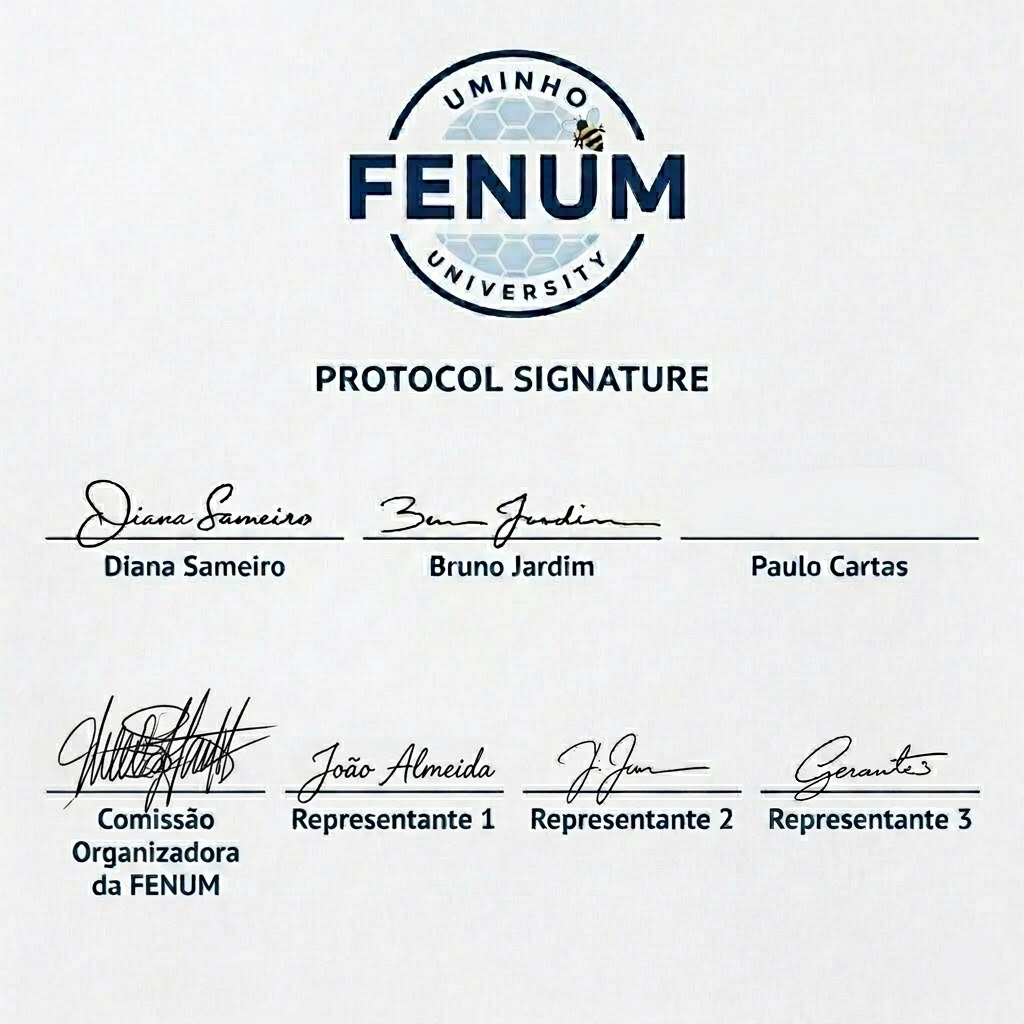
\includegraphics[width=0.7\textwidth]{images/ata1.jpeg}
    \caption{Ata 1}
    \label{fig:ata1}
\end{figure}

\newpage
\phantomsection
\subsection*{II. Ata da segunda reunião}
\addcontentsline{toc}{subsection}{II. Ata da segunda reunião}

\textbf{Data de realização:} 4 de março de 2026 \\
\textbf{Hora de início:} 09:45h \\
\textbf{Hora de término:} 12:00h

\textbf{Participantes}
\begin{itemize}[leftmargin=1.5cm]
    \item Bruno Jardim;
    \item Paulo Cartas;
    \item \textit{Ausência justificada:} Diana Sameiro (reunião externa com parceiros institucionais);
    \item Comissão Organizadora da FENUM;
    \item Equipa técnica do projeto.
\end{itemize}

\textbf{Contextualização}

Ao quarto dia do mês de março de dois mil e vinte e seis, realizou-se a
segunda reunião de trabalho, já numa fase de consolidação do levantamento
inicial. Esta sessão teve como propósito transformar as necessidades recolhidas
na reunião anterior em requisitos de descrição mais objetivos e verificáveis,
assegurando maior consistência na definição das entidades centrais do sistema.

No decorrer da reunião, foi reforçada a necessidade de uniformizar critérios de
registo e nomenclatura dos dados, de modo a reduzir ambiguidades e a preparar
uma base sólida para as etapas de modelação subsequentes.

\textbf{Tópicos abordados}

Nesta reunião foram discutidos e validados os requisitos de descrição do
sistema: identificação de estudantes, empresas, propostas, palestras, oradores,
bancas e respetivas relações de suporte ao evento.

\textbf{Levantamentos}

Ficou estabelecido que os estudantes devem possuir identificador único e dados
académicos essenciais, que as empresas devem ter identificação própria e que as
propostas devem ser associadas à entidade empregadora correspondente. Foi
igualmente aceite a necessidade de registar palestras com lotação, oradores,
bancas e sessões de \textit{speed interview}, assegurando suporte aos novos
requisitos de agenda e de consulta.

Adicionalmente, foi discutida a normalização mínima dos dados de contacto e
identificação, com vista a evitar duplicações e inconsistências. Foram
identificados campos obrigatórios, campos opcionais e regras preliminares de
validação para suportar integridade dos registos no momento da inserção e
atualização.

\textbf{Decisões}
\begin{itemize}[leftmargin=1.5cm]
    \item Aprovar os requisitos de descrição em versão preliminar para posterior
    tabelação no ponto 2;
    \item Preparar requisitos de manipulação centrados em consultas, gestão de
    estudantes, resultados de \textit{speed interviews}, atribuição de bancas e
    análises de procura;
    \item Agendar terceira reunião com foco em operações e controlo.
\end{itemize}

\textbf{Assinaturas} \\
\begin{figure}[h]
    \centering
    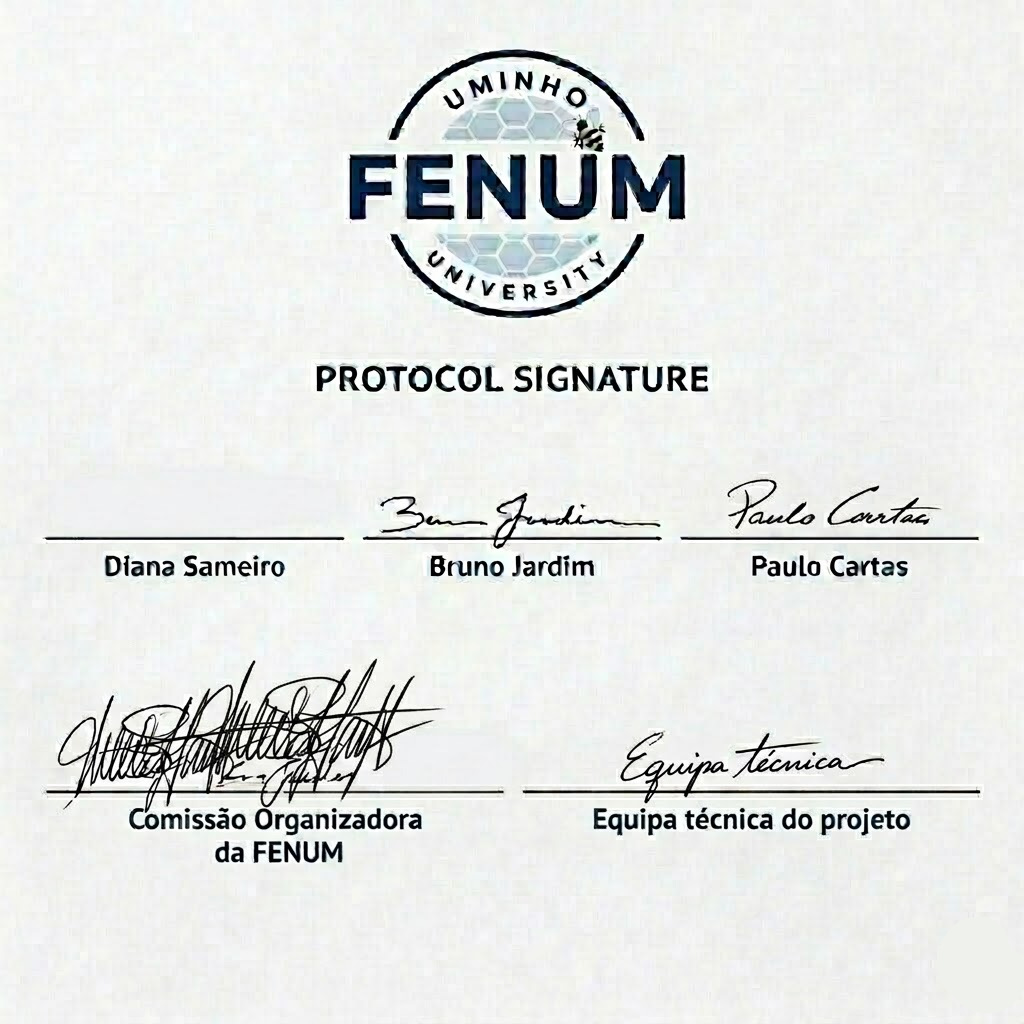
\includegraphics[width=0.7\textwidth]{images/ata2.jpeg}
    \caption{Ata 2}
    \label{fig:ata2}
\end{figure}

\newpage
\phantomsection
\subsection*{III. Ata da terceira reunião}
\addcontentsline{toc}{subsection}{III. Ata da terceira reunião}

\textbf{Data de realização:} 8 de março de 2026 \\
\textbf{Hora de início:} 09:10h \\
\textbf{Hora de término:} 11:40h

\textbf{Participantes}
\begin{itemize}[leftmargin=1.5cm]
    \item Diana Sameiro;
    \item Paulo Cartas;
    \item \textit{Ausência justificada:} Bruno Jardim (suporte operacional no recinto da feira);
    \item Comissão Organizadora da FENUM;
    \item Representantes de empresas parceiras.
\end{itemize}

\textbf{Contextualização}

Ao oitavo dia do mês de março de dois mil e vinte e seis, realizou-se a terceira
reunião, orientada para a componente operacional do sistema. Após a validação
preliminar dos requisitos de descrição, a equipa centrou-se na identificação das
operações críticas da FENUM e nas consultas/manipulações que deveriam suportar a
atividade diária do evento.

Esta sessão permitiu enquadrar cenários de utilização real, incluindo situações
de exceção, com o objetivo de garantir que os requisitos de manipulação e
segurança refletissem de forma fiel as necessidades práticas da organização.

\textbf{Tópicos abordados}

Foram discutidos os requisitos de manipulação e de controlo associados ao ciclo
operacional do evento: listagem de estudantes sem candidaturas, oradores com
múltiplas palestras, gestão de estudantes, resultado de \textit{speed
interviews}, consulta de empresas aprovadas, atribuição de bancas, agendas
diárias, consultas por empresa, procura de propostas e empresas sem
candidaturas.

\textbf{Levantamentos}

Concluiu-se que o sistema deve permitir consultar estudantes sem candidaturas,
listar oradores com mais de uma palestra, gerir estudantes, atualizar o
resultado de \textit{speed interviews}, consultar empresas aprovadas, atribuir e
consultar bancas, compor a agenda diária de um estudante, listar \textit{speed
interviews} por empresa, obter as propostas mais procuradas e identificar
empresas sem candidaturas.

No plano de segurança e integridade, ficou definido que as operações devem
respeitar validações de acesso, de duplicação, de lotação, de temporalidade do
resultado das entrevistas e de consistência entre empresa, proposta e banca.
Estes cenários serão refletidos nos requisitos de manipulação e controlo para
garantir comportamento previsível do sistema em situações reais de utilização.

\textbf{Decisões}
\begin{itemize}[leftmargin=1.5cm]
    \item Validar requisitos de manipulação e controlo como base para modelação;
    \item Registar histórico de operações relevantes para auditoria e consulta;
    \item Agendar reunião final de validação global dos requisitos.
\end{itemize}

\textbf{Assinaturas} \\
\begin{figure}[h]
    \centering
    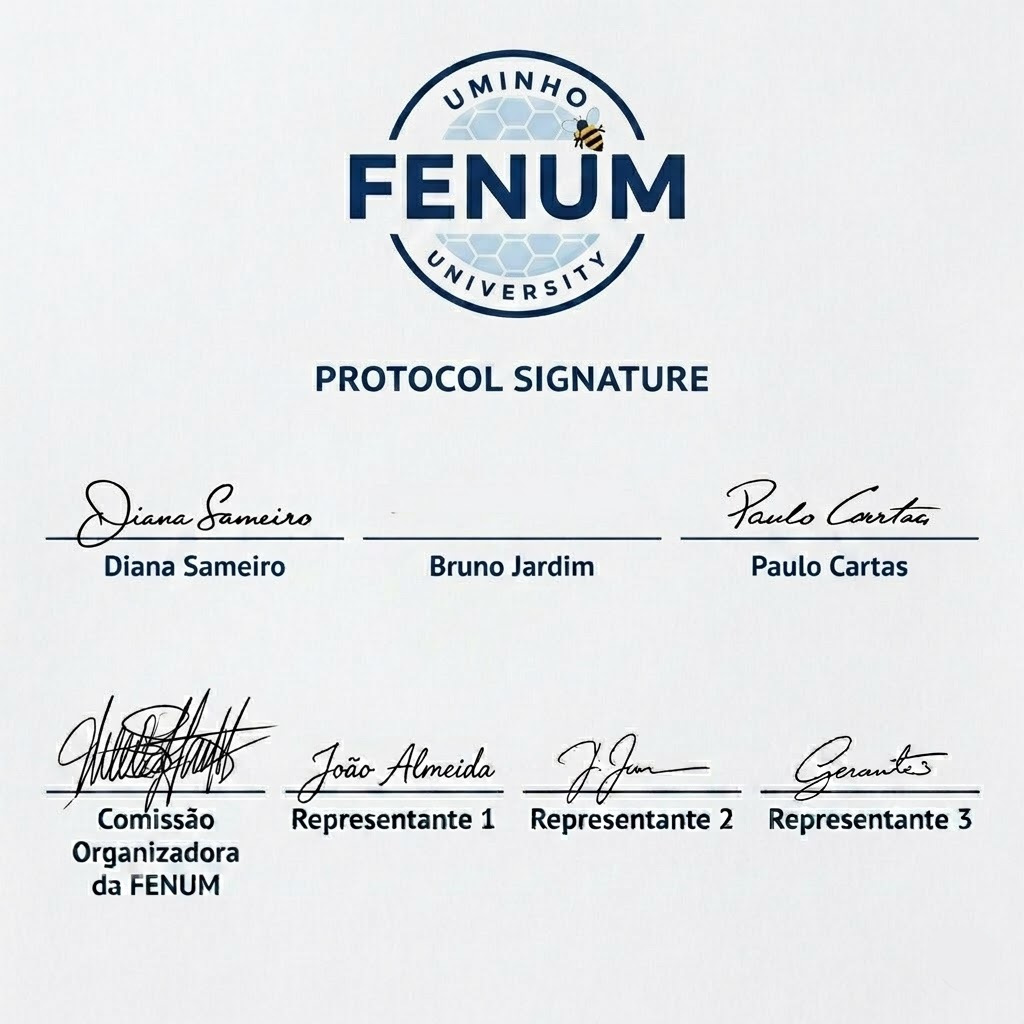
\includegraphics[width=0.7\textwidth]{images/ata3.jpeg}
    \caption{Ata 3}
    \label{fig:ata1}
\end{figure}


\newpage
\phantomsection
\subsection*{IV. Ata da quarta reunião}
\addcontentsline{toc}{subsection}{IV. Ata da quarta reunião}

\textbf{Data de realização:} 14 de março de 2026 \\
\textbf{Hora de início:} 09:20h \\
\textbf{Hora de término:} 11:55h

\textbf{Participantes}
\begin{itemize}[leftmargin=1.5cm]
    \item Diana Sameiro;
    \item Bruno Jardim;
    \item Paulo Cartas;
    \item Comissão Organizadora da FENUM;
    \item Equipa técnica do projeto;
    \item Representantes de empresas parceiras.
\end{itemize}

\textbf{Contextualização}

Ao décimo quarto dia do mês de março de dois mil e vinte e seis, realizou-se a
quarta reunião com caráter de validação final da fase de levantamento e análise
de requisitos. Nesta sessão, procedeu-se ao cruzamento das decisões tomadas nas
reuniões anteriores, com vista à confirmação da coerência global da solução
proposta.

O principal objetivo foi encerrar esta fase com um conjunto de requisitos
consistente, sem ambiguidades relevantes e devidamente rastreável, criando
condições para a transição para a modelação concetual.

\textbf{Tópicos abordados}

Nesta reunião final procedeu-se à revisão integral dos requisitos levantados,
validação de consistência entre itens e confirmação dos critérios de aceitação
para transição à modelação concetual. Foram validados os novos requisitos de
manipulação associados a consultas analíticas, gestão de estudantes, agenda,
resultados de entrevistas e atribuição de bancas.

\textbf{Levantamentos}

Foram removidas ambiguidades semânticas, alinhadas designações de entidades e
confirmadas as regras de integridade e permissões. O Departamento de Gestão de
Base de Dados da FENUM assumiu formalmente a responsabilidade de manter o
histórico de decisões e apoiar a validação das próximas fases do projeto.

Foi ainda validada a rastreabilidade entre origem do requisito, justificação
funcional e impacto esperado no modelo de dados. A equipa confirmou que os
requisitos de manipulação revistos cobrem consultas de ausência, agregação,
ordenamento, filtros por entidade, gestão de estado e restrições de lotação,
assegurando que o modelo lógico poderá refletir corretamente essas operações.

\textbf{Decisões}
\begin{itemize}[leftmargin=1.5cm]
    \item Aprovar a versão final dos requisitos para avançar para modelação concetual;
    \item Manter as atas e evidências de validação nos anexos do relatório;
    \item Definir revisões periódicas de qualidade dos dados nas fases seguintes;
    \item Confirmar que os novos requisitos de manipulação serão transpostos
    para consultas e operações físicas na fase de implementação.
\end{itemize}

\textbf{Assinaturas} \\
\begin{figure}[h]
    \centering
    
\includegraphics[width=0.7\textwidth]{images/assinaturas.jpeg}
    \caption{Ata 4}
    \label{fig:ata1}
\end{figure}


\newpage
\phantomsection
\subsection*{V. Evidências complementares de reuniões}
\addcontentsline{toc}{subsection}{V. Evidências complementares de reuniões}

\begin{itemize}[leftmargin=1.5cm]
    \item Registos de presença;
    \item Capturas de agenda e calendarização;
    \item Versões de trabalho dos requisitos antes e depois da validação.
\end{itemize}

\newpage
\phantomsection
\subsection*{VI. Requisitos consolidados após as reuniões}
\addcontentsline{toc}{subsection}{VI. Requisitos consolidados após as reuniões}

Após a consolidação das quatro reuniões, os requisitos foram estruturados de
forma final por tipo. A listagem seguinte apresenta os itens levantados e a
respetiva organização.

\textbf{A) Requisitos de descrição (levantados)}
\begin{itemize}[leftmargin=1.5cm]
    \item Registar estudante com identificador único, nome, contacto, curso,
    universidade e ano letivo;
    \item Registar entidade empregadora com identificador único, nome e setor de
    atividade;
    \item Registar proposta com tipo (estágio/emprego/projeto), descrição,
    perfil procurado e empresa associada;
    \item Registar banca por empresa no recinto da feira;
    \item Registar sessão de entrevista rápida com data/hora e intervenientes.
\end{itemize}

\textbf{B) Requisitos de manipulação (levantados)}
\begin{itemize}[leftmargin=1.5cm]
    \item Permitir candidatura de estudante a proposta;
    \item Permitir atualização de estado da candidatura pela entidade
    empregadora;
    \item Permitir criação, alteração e cancelamento de entrevistas rápidas;
    \item Permitir registo e gestão de inscrições em palestras;
    \item Permitir consultas de lotação atual e lotação máxima por sessão;
    \item Permitir extração de indicadores de procura (ex.: propostas mais
    procuradas).
\end{itemize}

\textbf{C) Requisitos de controlo (levantados)}
\begin{itemize}[leftmargin=1.5cm]
    \item Definir perfis de acesso distintos (organização, empresa, estudante,
    staff técnico);
    \item Restringir acesso das empresas aos dados estritamente necessários ao
    processo de recrutamento;
    \item Registar histórico de operações críticas para auditoria;
    \item Aplicar validações de integridade nos registos obrigatórios;
    \item Prever regras de prevenção de conflitos de agenda e sobrelotação.
\end{itemize}

\textbf{D) Mapeamento para rastreabilidade}

Para garantir a rastreabilidade na secção 2, cada requisito foi associado aos
seguintes campos: tipo, número, data, descrição do requisito, fonte e analista.

\begin{itemize}[leftmargin=1.5cm]
    \item Fonte: atas I, II, III e IV e documentação de apoio;
    \item Data: data da reunião onde o requisito foi definido ou validado;
    \item Analista: elemento(s) da equipa responsável pela redação final.
\end{itemize}

\end{document}
